\documentclass[a4paper,12pt,floatssmall]{scrartcl}

% Page geometry's formatting
\usepackage[left=2.5cm,right=2.5cm,top=2.5cm,bottom=2.5cm]{geometry}
\usepackage{indentfirst}
\usepackage{placeins}
\usepackage{float}
% Language-specific settings
\usepackage[T1]{fontenc}
\usepackage[utf8]{inputenc}
\usepackage[polish]{babel}
\usepackage{polski}
% Elements' embedding
\usepackage{listings}
\usepackage{graphicx}
\usepackage[bf]{caption}
\usepackage{subcaption}
\usepackage{hyperref}
\usepackage{array}
\usepackage{tabularx}
\usepackage{longtable}
\usepackage[table,xcdraw]{xcolor}
% Text-formatting
\usepackage[autostyle]{csquotes}
\usepackage{caption}
\usepackage{moresize}
\usepackage{amsmath}
% Miscellaneous
\usepackage[backend=biber,style=ieee]{biblatex}
% \usepackage[enable]{easy-todo}
\usepackage{lipsum}
\usepackage{setspace}

% ================================================================================================================================== %
% --------------------------------------------------------- Configuration ---------------------------------------------------------- %
% ================================================================================================================================== %

% Unordered list
\renewcommand{\labelitemi}{\textbullet}

% Bibliography file
\addbibresource{bibliography.bib}

% ================================================================================================================================== %
% ------------------------------------------------------- Macrodefinitions --------------------------------------------------------- %
% ================================================================================================================================== %

% Redefininiton of the title page
\renewcommand{\maketitle}{
\begin{titlepage}
    \vfill
    \begin{center}
        \begin{figure}
            \centering
            
\includegraphics[scale=0.9]{img/header.png}
            \vspace{0.5cm}
        \end{figure}
    \end{center}
    \vspace{2cm}
    \begin{center}
        {\HUGE {\textbf{Programowanie kładów FPGA}}}\\
        \vspace {0.4cm}
        {\Large {(projekt)}}
    \end{center}
    \vspace{4cm}
    \begin{center}
        {\setstretch{1.5}\textbf{\LARGE Implementacja algorytmów cyfrowego przetwarzania sygnałów audio na bazie układu FPGA z interfejsem UART}}
        \vspace{3cm}
    \end{center}
    \vfill
    \begin{center}
        {\textbf{\normalsize Pierczyk Krzysztof}}
    \end{center}
    \vfill
    \begin{center}
        \large{Warszawa, \today \par}
    \end{center}
\end{titlepage}
}

% Definition of `part` module
\renewcommand\partheadstartvskip{\clearpage\null\vfil}
\renewcommand\partheadmidvskip{\par\nobreak\vskip 20pt\thispagestyle{empty}}
\renewcommand\partheadendvskip{\vfil\clearpage\setcounter{section}{0}}
\renewcommand\raggedpart{\centering}

% ================================================================================================================================== %
% ------------------------------------------------------------- Text --------------------------------------------------------------- %
% ================================================================================================================================== %

\begin{document}
    
% Title
\maketitle

% Table of content
\tableofcontents

% Chapter I - Theoretical analysis
\part{Analiza teoretyczna}
\section{Wstęp}

Celem projektu jest opracowanie i~zaimplementowanie zestawu wybranych metod przetwarzania sygnałów audio znanych z~popularnych multiefektów gitarowych. Zadaniem tego typu rozwiązań jest modyfikowanie próbkowanego dźwięku w~czasie rzeczywistym w taki sposób, aby urozmaicić jego brzmienie np. poprzez modulację, przesunięcie fazowe lub wprowadzenie dodatkowych składowych. Przykładami takich efektów są m.in.

\begin{itemize}
    \item \textbf{echo} (opóźnienie, ang. \textit{delay}) - do sygnału dodawana jest jedna lub kilka jego kopii opóźnionych o~określoną liczbę próbek; efekt ma symulować warunki panujące w~halach widowiskowych
    \item \textbf{overdrive} - nazwa ogółu metod prowadzących do znacznego zniekształcenia sygnału bazowego; jednym z~popularnych sposobów jego implementacji jest nałożenie obustronnych ograniczeń na wyjściowe wartości przepuszczanego sygnału
    \item \textbf{flanger} - kolejny efekt wykorzystujący opóźnione próbki sygnału; w~tym przypadku wielkość opóźnienia podlega cyklicznym zmianom, co przekłada się na pulsacyjny charakter wyjściowego dźwięku
    \item \textbf{tremolo} - efekt modulujący amplitudę sygnału zgodnie z~przebiegiem pewnej funkcji okresowej (np. sinus lub fala trójkątna); jego celem jest symulowanie rodzaju artykulacji polegającego na szybkim wydobywaniu dźwięków o~tej samej częstotliwości (np. poprzez szybkie szarpanie pojedynczej struny gitarowej) 
\end{itemize}

Powyższe efekty stanowią jedynie niewielki wycinek stosowanych rozwiązań, wśród których wymienić można także szeroko pojęte metody equalizacji, czy modyfikowania częstotliwości sygnału. Minimalna wersja projektu zakłada implementację scharakteryzowanych metod przetwarzania wraz z~prostymi mechanizmami wprowadzania i~wyprowadzania danych z~urządzenia a~także dostosowywania parametrów filtrów. Jako metodę komunikacji wybrano popularny (choć może w~niec innych zastosowaniach) interfejs UART (ang. \textit{universal asynchronous receiver-transmitter}). Jego prostota umożliwi przyspieszenie procesu implementacji, a~co za tym idzie szybsze przejście do zasadniczej części projektu. Cyfrowy charakter UARTa pozwoli w~przyszłości przejść na popularny interfejs $I^{2}S$, dzięki któremu możliwe będzie proste dołączenie do urządzenia układów przetwornikowych. Testowanie urządzenia obywać się będzie z~pomocą prostej aplikacji w~języku Python, która za pośrednictwem wirtualnego portu szeregowego wysyłać będzie do urządzenia próbki dźwięku. Sygnał wychodzący z~układu FPGA będzie następnie odtwarzany za~pomocą jednej z~wielu dostepnych w~Pythonie bibliotek audio jak np. \verb|pyaudio|.

\section{Analiza interfejsu komunikacyjnego}

Interfejs UART jest dzisiaj dostępny w~niemal wszystkich obecnych na mikrokontrolowerowych oraz w~wielu układach typu SoC. Jego popularność wynika zarówno z~(jak sama nazwa wskazuje) uniwersalnego charakteru jak i~prostoty implementacji. UART to cyfrowe urządzenie peryferyjne umożliwiające szeregową komunikację asynchroniczną. W~większości implementacji parametry komunikacji takie jak szybkość, czy format danych mogą być konfigurowane poprzez zmianę wartości odpowiednich rejestrów sterujących. Nierzadko możliwe jest też ustawienie trybu komunikacji spośród \textit{simplex}, \textit{duples} lub ~\textit{half-duples}. Interfejsy tego typu, szczególnie w~zastosowaniach przemysłowych, są często sprzęgane z~konwerterami poziomów logicznych odpowiednich dla standardów RS-232 lub RS-485.

\begin{figure}
    \centering
    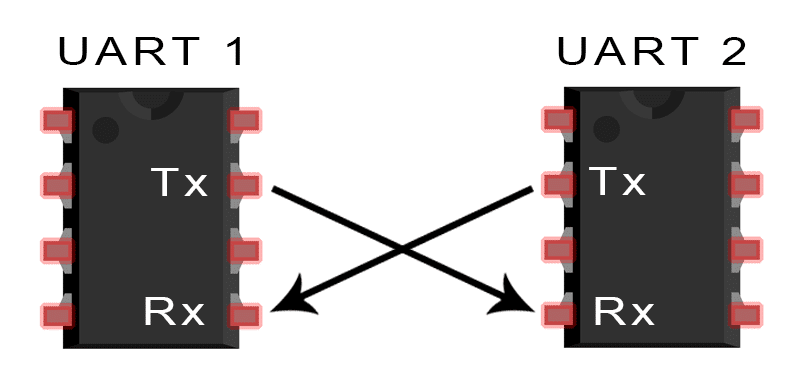
\includegraphics[scale=0.5]{img/uart.png}
    \captionsetup{format=plain,justification=centering}
    \caption{Typowa struktura komunikacji dwóch węzłów z~wykorzystaniem układu UART, źródło: \cite{uart}}
    \label{UART}
\end{figure}

Komunikacja asynchroniczna wymaga aby wszystkie węzły nadawały i~odbierały dane o~z~góry ustalonym formacie i~długości znaku (wynikającym z~szybkości transmisji). Ponadto należy wziąć pod uwagę, że zegary obecne w~poszczególnych urządzeniach mogą się z~czasem rozsynchronizowywać, a~co za tym idzie konieczny jest mechanizm ponownej synchronizacji. W~przypadku komunikacji z~wykorzystaniem modułu UART mechanizm ten wynika z~formatu przesyłanych danych. Typowa ramka składa się z~trzech elementów: \textbf{bitu startu}, \textbf{bitów danyc} oraz \textbf{bitów stopu}. Bit startu oznacza początek nowej ramki i~jest sygnalizowany stanem niskim na linii. Po nim następować może pewna liczba bitów danych - zazwyczaj $7$ lub $8$  - a~na końcu jeden lub dwa bity stopu (sygnalizowane stanem wysokim). Bit startu odpowiada za synchronizację zegarów wykorzystywanych do próbkowania stanu linii, natomiast bity stopu definiują minimalną przerwę między kolejnymi ramkami. Fakt że każdy bit startu to ponowna okazja do zsynchronizowania zegarów sprawia, że nie muszą one pracować z~dokładnie tymi samymi szybkościami. Niewielkie różnice nie powodują błędów w~odbiorze danych.

\begin{figure}
    \centering
    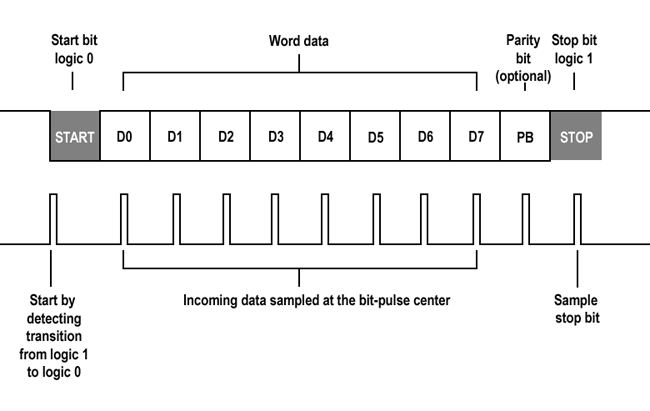
\includegraphics[scale=0.5]{img/uart_frame.png}
    \captionsetup{format=plain,justification=centering}
    \caption{Struktura ramki UART, źródło: \cite{uart_frame}}
    \label{UART}
\end{figure}

Format ramki może zostać rozszerzony o~element kontrolny w~postaci \textbf{bitu parzystości}. Jeśli występuje, przyjmuje on wartość zależną od ilości bitów w~stanie wysokim w~przesyłanych danych i~znajduje się przed bitami stopu. Możliwy jest bit parzystości (ang. \textit{even}) - ustawiony, gdy suma jest parzysta - lub nieparzystości (ang. \textit{odd}) - ustawiany, gdy suma jest nieparzysta. Dodatkowy element pozwala wykrywać ewentualne błędy transmisji. Format ramki często oznacza się w~postaci trzyznakowego identyfikatora postaci $DPS$, gdzie $D$ oznacza ilość bitów danych, $P$ - typ bitu kontrolnego ($E$ - bit parzystości, $O$ - bit nieparzystości, $N$ - brak bitu kontrolnego) a~$S$ ilość bitów stopu. Typowowymi prędkościami transmisji przez UART są:

\begin{itemize}
    \item 9600 bit/s
    \item 19200 bit/s
    \item 38400 bit/s
    \item ...
\end{itemize}

Jest to pewna zaszłość historyczna wynikająca z~częstotliwości standardowych oscylatorów dostępnych na rynku. Moduły współcześnie implementowane w~układach scalonych wzbogacone są często o~dodatkowe wyprowadzenia zegarowe umożliwiające komunikację synchroniczną. Tego typu urządzenia określane są zazwyczaj mianem USART (ang. \textit{universal synchronous asynchronous receiver-transmitter}).

% ================================================================================================================================== %
% ------------------------------------------------------------ Effects ------------------------------------------------------------- %
% ================================================================================================================================== %

\section{Efekty dźwiękowe}

Pierwszą decyzją projektową dotyczącą efektów było stworzenie jednolitego interfejsu implementaowanych bloków przetwarzających. Ma to umożliwić arbitralne połączenie ich w~potok oraz dodanie w~przyszłości nowych efektów bez wprowadzania znacznych zmian w~projekcie. Wykorzystano w~tym celu strukturę zaczerpniętą z~\cite{fpga_pedal}, która została przedstawiona na Rys.\ref{effects-pipe}.

\vspace{0.5cm}
\begin{figure}[ht]
    \centering
    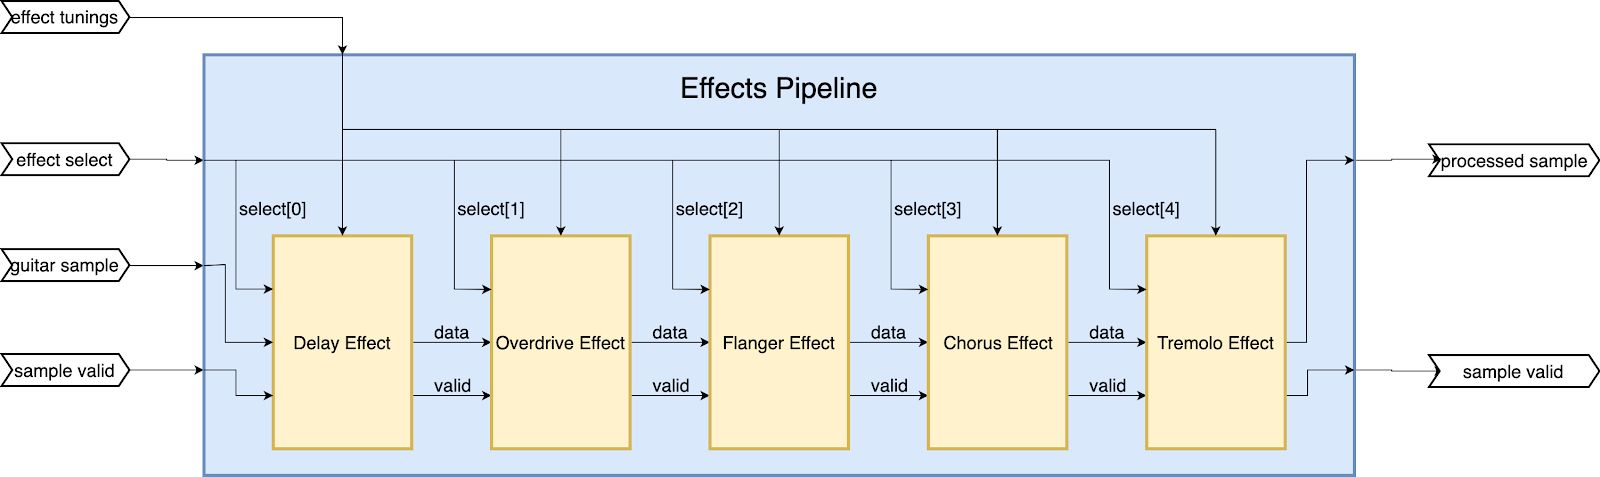
\includegraphics[scale=0.25]{img/pipe.jpg}
    \captionsetup{format=plain,justification=centering}
    \caption{Planowana struktura potoku efektów, źródło: \cite{fpga_pedal}}
    \label{effects-pipe}
\end{figure}
\vspace{0.5cm}

Każdy blok posiada trzy standardowe wejścia oraz dwa standardowe wyjścia. Projekt zakłada wykorzystanie 16-bitowych próbek dźwięku, co determinuje szerokość szyn danych. Wejścia \verb|valid| aktywowane są zboczem narastajacym i~oznaczają pojawienie się nowej próbki na wejściu bloku. Po przetworzeniu próbki moduł ma obowiązek wystawienia danych na linię wyjściową oraz wygenerowanie zbocza narastającego na wyjściu \verb|valid|, które podłączone jest do odpowiadającego wejścia następnego modułu. Każdy z~bloków posiada także jednobitowe wejście \verb|enable|. Stan niski na tej linii oznacza, że blok powinien przekazywać na swoje wyjście próbkę wejściową bez jej modyfikowania. Każdy blok może dodatkowo implementować arbitralne wejścia konfiguracyjne specyficzne dla działania danego algorytmu. W~przypadku blok \textit{overdrive} może być to na przykład 8-bitowa wartość wzmocnienia sygnału i~16-bitowe wartości górnego i~dolnego nasycenia (szczegóły opisano w~dalszej części dokumentu).

Tak zaprojektowana struktura pozwala w~łatwy sposób modyfikować obecne w~systemie efekty oraz nie nakłada ścisłych ograniczeń na interfejs użytkownika wykorzystywany do ich kontrolowania. Również sposób dostarczania i~odbierania danych z~potoku nie jest dzięki temu ograniczony do konkretnego interfejsu komunikacyjnego.

% ----------------------------------------------------------- Overdive ------------------------------------------------------------- %

\subsection{Overdrive}

Jak nakreślono we wstępie efekt przesterowania (ang. \textit{overdive}) określa zespół metod prowadzących do znacznego zniekształcenia sygnału bazowego poprzez dodanie do niego dodatkowych składowych harmonicznych. Częstym sposobem implementacji takiego efektu jest obustronne przycinanie sygnału wejściowego. W~niniejszym projekcie zastosowana zostanie struktura przedstawiona na Rys. {effects-overdrive}.

\vspace{0.5cm}
\begin{figure}[ht]
    \centering
    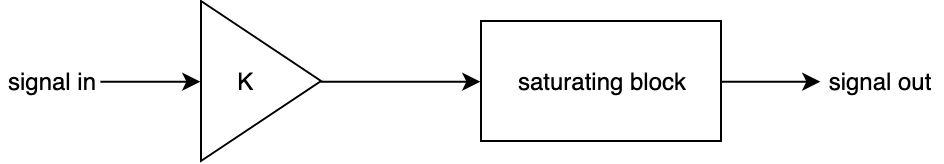
\includegraphics[scale=0.4]{img/overdrive.jpg}
    \captionsetup{format=plain,justification=centering}
    \caption{Schemat bloku \textit{overdrive}, źródło: \cite{fpga_pedal}}
    \label{effects-overdrive}
\end{figure}
\vspace{0.5cm}

Pierwszym etapem przetwarzania jest tutaj wzmocnienie sygnały wejściowego o~wartość kontrolowaną przez rejestr wejsciowy bloku. Zakres potencjalnego wzmocnienia zostanie ustalony na etapie testowania układu. Będzie ono realizowane poprzez 16-bitowe mnożenie z~nasyceniem. Wzmocniony sygnał zostaje następnie przepuszczony przez blok nasycenia. Jeżeli jego wartość mieści się pomiędzy skonfigurowanymi poziomami zostaje on podany na wyjście bez dalszych modyfikacji. W~przeciwnym wypadku na wyjściu pojawia się odpowiednia wartość nasycenia. Funkcjonalność ta może zostać zaimplementowana przy użycia dwóch 16-bitowych komparatorów oraz multipleksera.

% ------------------------------------------------------------ Delay --------------------------------------------------------------- %

\subsection{Delay}

Efekt pogłosu uzyskiwany jest poprzez sumowanie przychodzących próbek z~próbkami opóźnionymi o~określoną liczbę cykli. Realizacja takiego bloku może bazować na filtrze typu FIR (ang. \textit{Finite Impulse Response}) lub IIR (ang. \textit{Infinite Impulse Response}). W~przypadku pierwszego z~nich przeszłe próbki są opóźnionymi wersjami \textbf{sygnału wejściowego}. Liczba próbek sumowanych może być stała lub parametryzowana. Drugi sposób implementacji przewiduje sumowanie pórbki wejściowej jedynie z~jedną wersją opóźnioną sygnału. Wersja ta jest jednak pobierana z~\textbf{wyjścia układu}, co oznacza, że jest ona zależna od wszystkich poprzednich próbek sygnału. Właśnie to rozwiązanie zostanie zastosowane w~niniejszym projekcie. Jego struktura została przedstawiona na Rys.\ref{effects-delay}. W~celu uzyskania stabilnego układu konieczne jest wprowadzenia tłumienia sygnału opóźnionego. Kierując się informacjami zawartymi w~\cite{fpga_pedal} wartości tego tłumienia przyjęto w~zakresie od $0$ do $0.5$. W~celu otrzymania takiego zakresu wyjście z~bloku mnożącego będzie przepusówane o~8~bitów w~prawo (tj. dzielone przez 256).

\vspace{0.5cm}
\begin{figure}[ht]
    \centering
    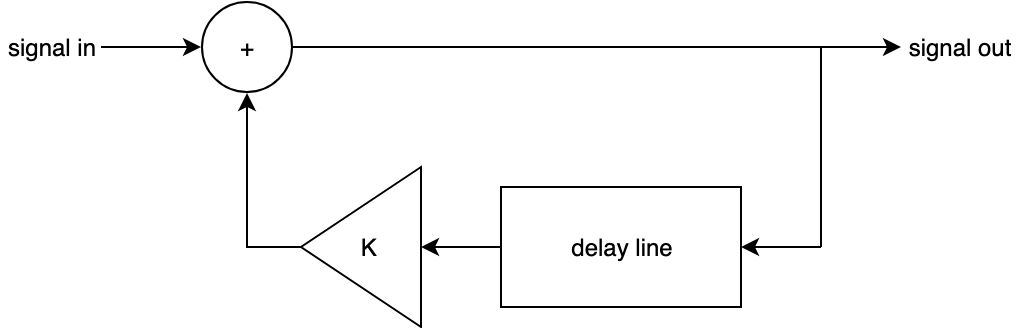
\includegraphics[scale=0.4]{img/delay.jpg}
    \captionsetup{format=plain,justification=centering}
    \caption{Schemat bloku \textit{delay}, źródło: \cite{fpga_pedal}}
    \label{effects-delay}
\end{figure}
\vspace{0.5cm}

Od strony technicznej implementacyja takiego bloku wymaga układu mnożącego, kolejki typu FIFO oraz multipleksera. Siła tłumienia echa ustalana jest poprzez wartość jednego z~wejść do układu mnożącego. Głębokość echa definiuje z~kolei indeks rejestru w~kolejce, którego wartość wystawiana jest na wyjście modułu opóźniającego. Oba parametry efektu regulowane będą przez rejestry wejściowe bloku. Maksymalna głębokość kolejki zostanie ustalona na etapie testowania.

% ----------------------------------------------------------- Flanger -------------------------------------------------------------- %

\subsection{Flanger}

\textit{Flagner} jest efektem, którego brzmienie trudno opisać, jednak zasada jego działania jest stosunkowo prosta. Efekt ten powstaje poprzez nałożenie na sygnał filtru grzebieniowego, którego charakterystyka amplitudowa wykonuje sinusoidalne oscylacje w~okół ustalonego punktu. W~prakyce układ taki realizuje się poprzez sumowanie sygnału z~jego opóźnionymi (nieprzetworzonymi) wersjami. Wartość tego opóźnienia jest jednak okresowo zmienna. Struktura takiego rozwiązania przedstawiona została na Rys.\ref{effects-flanger}. Aby kontrolować siłę efektu do ukłądu wprowadzone zostaną dodatkowe bloki tłumienia. Ich wartość zawierać się będzie w~przedziale od $0$~do $1$, natomiast ich suma będzie stale równa $1$. Podobnie jak w~przypadku pogłosu wykorzystywana głębokość kolejki FIFO (a~tym samym efektywna amplituda oscylacji wartości opóźnienia) będzie ustalana porpzez zewnętrzny parametr.

\vspace{0.5cm}
\begin{figure}[ht]
    \centering
    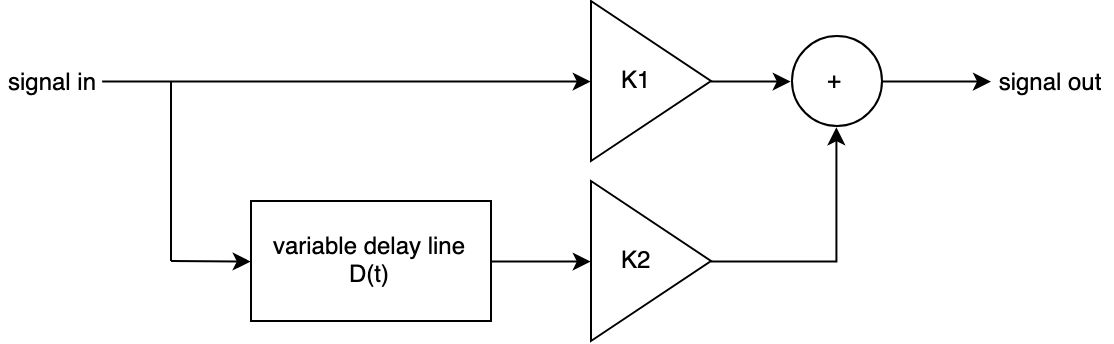
\includegraphics[scale=0.4]{img/flanger.jpg}
    \captionsetup{format=plain,justification=centering}
    \caption{Schemat bloku \textit{flanger}, źródło: \cite{fpga_pedal}}
    \label{effects-flanger}
\end{figure}
\vspace{0.5cm}

Implementacja efektu będzie wykorzystywac bloki stworzone podczas realizacji poprzedniego efektu takie jak układy mnożące oraz kolejka FIFO. Dodatkowym elementem będzie tutaj generator funkcji sinus o~zmiennej częstotliwości. Czestotliwość ta będzie również ustalana poprzez zewnętrzny parametr.

% ----------------------------------------------------------- Tremolo -------------------------------------------------------------- %

\subsection{Tremolo}

Efekt tremolo uzyskuje się poprez modulację amplitudy sygnału wejściowego. Jest to realizowane poprzez mnożenie sygnału z~pewną funkcją okresową jak np. sinus lub fala trójkątna. W~projekcie zaimplementowane zostaną oba rodzaje modulacji. Po wykonaniu testów wybrany zostanie ten, który będzie pozwalał uzyskać ciekawsze brzmienie. Schemat blokowy rozwiązania został przedstawiony na Rys.\ref{effects-tremolo}. Podobnie jak w~przypadku pogłosu wykorzystane zostanie tu 8-bitowe przesówanie wyniku mnożenia celem uzyskania efektywnej amplitudy fali modulującej w~zakresie od $0$ do $1$ (przy załżeniu, że wyjście z~generatora fali ma wartość 8-bitową).

\vspace{0.5cm}
\begin{figure}[ht]
    \centering
    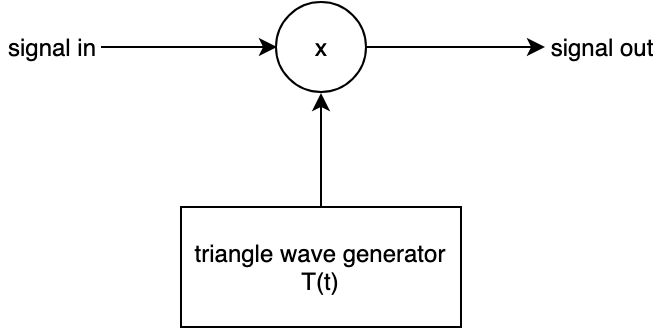
\includegraphics[scale=0.4]{img/tremolo.jpg}
    \captionsetup{format=plain,justification=centering}
    \caption{Schemat bloku \textit{tremolo}, źródło: \cite{fpga_pedal}}
    \label{effects-tremolo}
\end{figure}
\vspace{0.5cm}
% ================================================================================================================================== %
% ---------------------------------------------------------- Interface ------------------------------------------------------------- %
% ================================================================================================================================== %

\section{Interfejs użytkownika}

Ostatnim elementem projektu jest zaimplementowanie wygodnego interfejsu użytkownika. Powinien on umożliwiać niezależną aktywację każdego z~efektów oraz pozwalać na regulowanie ich parametrów. Układ FPGA udostępniać będzie cztery wejścia cyfrowe (przyciski). Zostaną one podłączone (za pośrednictwem przerzutników) do wejść \verb|enable| poszczególnych bloków przetwarzających. Aktywacja efektu możliwa będzie dzięki zmianie stanu przełącznika. Kontrola parametrów bloków przetwarzana zostanie zrealizowana za pomocą potencjometrów. Ich interfejs może zostać stworzony na dwa sposoby. Ostateczny wybór zostanie podjęty po głęszbym przeanalizowaniu zagadnienia. 

Pierwszym pomysłem jest wykorzystanie modułu XADC od Xilinx. Pozwoliłoby to na podłączenie wszystkich potencjometrów do układu FPGA z~wykorzystaniem multipleksera analogowego (np. CD74HC4067), którego wejście przełączane byłoby z~pewną częstotliwością przez układ sterujący. Wymagałoby to jednak wykorzystanie gotowego bloku IP oraz stworzenia odpowiedniego interfejsu od strony aplikacji.

Drugim pomysłem jest wdrożenie dodatkowego modułu UART, który komunikowałby się z~zewnętrznym mikrokontrolerem realizującym pomiar napięć na potencjometrach poprzez wbudowane kanały przetwornika A/C. W~takim przypadku układ FPGA odpytywałby podrzędny względem niego mikrokontroler w~sposób cykliczny, pozyskując cyfrowe wartości orientacji potencjometrów. Niezależnie od wyboru metody cyfrowe wartości pomiarów zostaną podłączone poprzez przerzutniki do wejśc konfiguracyjnych odpowiendich bloków przetwarzających sygnały.

% ================================================================================================================================== %
% --------------------------------------------------------- Simulations ------------------------------------------------------------ %
% ================================================================================================================================== %

\section{Planowane symulacje}

Planowane symulacje można podzielić na dwie zasadnicze kategorie. Pierwsza z~nich obejmuje proste testy jednostkowe \textbf{w~skali mikro}. Mowa tu o~modułach takich jak generator taktowania dla UARTa, układ mnożący, czy generator fali trójkątnej wykorzystywany w~algorytmach przetwarzania sygnału. Każdemu z~tych elementów powinien odpowiadać prosty podprojekt typu \textit{testbench}, który weryfikuje poprawność jego działania. Chociaż tworzenie tak drobnych elementów symulacyjnych może być do pewnego stopnia uciążliwe przy większej ilości testowanych elementów, to jednak doświadczenie pochodzące z~programowania pokazuje, że pozwala to zapobiec eskalacji wpływu drobnych błędów na działanie systemu jako całości.

Drugą kategorią symulacji będą testy systemowe sprawdzające \textbf{makroskopowe} działanie poszczególnych bloków funkcjonalnych. Tutaj również każdy z~modułów powinien otrzymać dedykowany projekt testowy. W~tym przypadku poza poprawnością działania podsystemów zostanie również zweryfikowana ich wydajność. Oszacowanie czasów przetwarzania danych przez dany blok funkcjonalny oraz jego złożoność przestrzenna (wymagana liczba zasobów układu FPGA) pozwolą z~jednej strony określić warunki krańcowe ich funkcjonowania, a~z~drugiej oszczować potencjalne możliwości rozwoju systemu np. o~dodatkowe efekty.

% ================================================================================================================================== %
% ------------------------------------------------------------ Tests --------------------------------------------------------------- %
% ================================================================================================================================== %

\section{Planowane testy}

Pierwszym testem poprawności działaniu układu będzie oczywiście empiryczna ocena dźwięku uzyskanego za pomocą poszczególnych efektów. Pozwoli ona nie tylko wykryć potencjalne błędy w~algorytmach przetwarzania (objawiające się np. wprowadzaniem nadmiernego szumu), ale także dostosować stałe parametry układu takie jak długości zastosowanych kolejek FIFO. 

Drugi krok weryfikacji rozwiązania zostanie zrealizowany dzięki zastosowanemu interfejsowi danych w~postaci aplikacji języka Python. Fakt, że posiadać będzie ona dostęp zarówno do surowych jak~i przetworzonych danych pozwoli w~łatwy sposób wyrysować wykresy przedstawiające przebiegi sygnałów i~np. ich transformaty. Możliwe będzie dzięki temu dokładne przyjrzenie się efektom działania poszczególnych filtrów celem wykrycia źródeł potencjalnych problemów. 

% ================================================================================================================================== %
% ----------------------------------------------------------- Platform ------------------------------------------------------------- %
% ================================================================================================================================== %

\section{Wybór platformy}

Ostateczny wybór platformy zostanie dokonany po stworzeniu fundamentów projektu pozwalających oszacować wymagania urządzenia dotyczące zasobów układu FPGA. Na ten moment potencjalny wybór został zawężony do trzech zestawów ewaluacyjnych. Pierwszy z~nich to \textbf{Digilent Cmod A7} wyposażony w~moduł XC7A35T-1CPG236C z~rodziny Artix-7. Niewielkie rozmiary oraz cena nieprzekraczająca 400zł są największymi zaletami tego wariantu. Został on wyposażony w~8-bitową pamięć SRAM o pojemności 512KB oraz pamięć szeregową Quad-SPI wielkości 4MB. Druga z~rozważanych platform to \textbf{Digilent Arty S7}. Jest to układ bardziej rozbudowany od poprzedniego. Posiada on na pokładzie moduł XC7S50-1CSGA324C (Spartan-7) zawierający ponad $50\%$ więcej bloków logicznych. Sama płytka oferuje ponadto kilka diod LED, przełączników mono- i~bistabilnych oraz cztery złącza Pmod. Cena tej platformy jest o~około $18\%$ wyższa, co oznacza wysoki stosunek zasobów do ceny, jednak liczyć się trzeba ze znacznie większymi wymiarami płytki.

Trzecim wariantem jest z~kolei zestaw \textbf{Digilent Cora Z7}. Jest to układ najuboższy w~bloki logiczne a~przy tym wyceniany na podobnym poziomie co Arty S7. Posiada on jednak układ XC7Z007S-1CLG400C z~rodziny Zynq co oznacza, że poza modułem FPGA zawiera on również jednordzeniowy procesor w~architekturze ARM Cortex-A9. Zestaw ten brany jest pod uwagę jedynie ze względu na prywatną sympatię autora do mikrokontrolerów bazujących na architekturze Cortex-M i~wynikającej z~niej chęci zapoznania się z~architekturą aplikacyjną rodziny ARM. Wariant ten zostanie wybrany wówacz, jeżeli zasoby zawartego w~nim modułu FPGA okażą się wystarczające do zaimplementowania tworzonego rozwiązania.


\part{Implementacja}
\section{Struktura projektu}

\vspace{0.5cm}
\begin{figure}[ht]
    \centering
    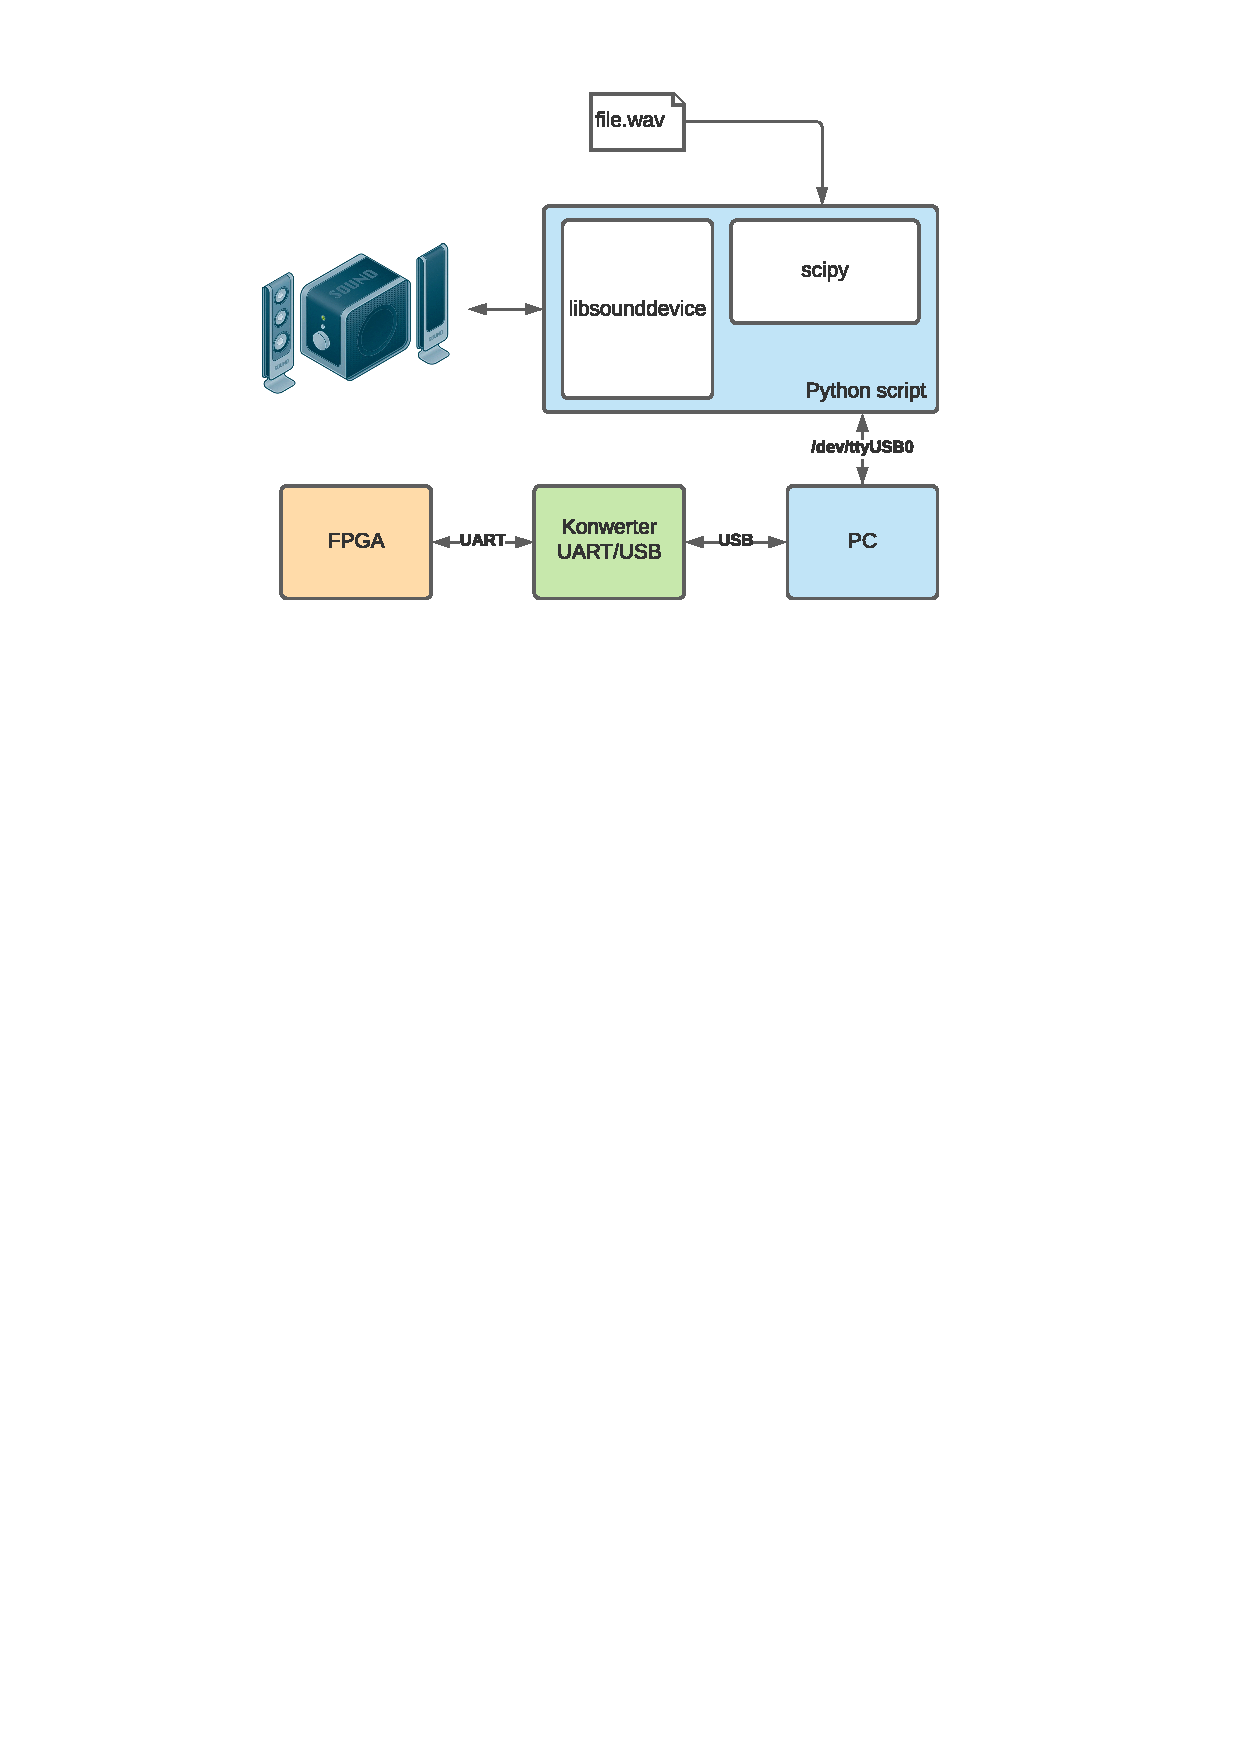
\includegraphics[scale=0.75]{img/diagrams/system.pdf}
    \captionsetup{format=plain,justification=centering}
    \caption{Struktura systemowa projektu}
    \label{system-structure}
\end{figure}
\vspace{0.5cm}

Realizację przedstawionej w~części pierwszej koncepcji rozpoczęto od nakreślenia struktury projektu na trzech płaszczyznach: \textbf{systemowej}, \textbf{implementacyjnej} i~\textbf{projektowej}. Pierwsza z~nich obejmowała zdefiniowanie węzłów, które będą brały udział w~procesie przetwarzania dźwięku od otwarcia zawierajacego go pliku do chwili wyemitowania przetworzonej wersji przez urządzenie audio. Jak przedstawiono na Rys. \ref{system-structure}, wyróżniono cztery zasadnicze jednostki. \textit{Skrypt języka Python} odpowiedzialny jest za załadowanie pliku dźwiękowego do pamięci RAM, przekazanie i~odebranie go z~układu przetwarzającego, a~także wysterowanie domyślnego urządzeni audio w~oparciu o~zmodyfikowane próbki. Urządzeniem przetwarzającym jest oczywiście układ \textit{FPGA}, który implementuje wymienione wyżej filtry. Pośrednikami w~komunikacji pomiędzy układem scalonym a~aplikacją są oparty o~układ FT232R \textit{mostek USB/UART} oraz \textit{komputer klasy PC}. Taka konfiguracja pozwala na dwukierunkową transmisję danych z~prędkością do 375KB na sekundę, co przy założeniu 16-bitowych próbek oraz częstotliwości próbkowania na poziomie 44100Hz powinno wystarczyć do strumieniowania dźwięku zarówno w~trybie mono jak i~stereo. W~projekcie wykorzystano biblioteki \verb|sounddevice| oraz \verb|scipy| języka Python. Pierwsza z~nich udostępnia interfejs dla szerokiej gamy urządzeń audio, natomiast druga pozwala przetwarzać pliki w~formacie WAV do postaci tablic danych biblioteki \verb|numpy|. Aby zredukować czas wykonywania operacji na wirtualnym porcie szeregowym, zdecydowano się podzielić strumieniowane dane na bloki o~wielkości 5000B, które wysyłane są do układu FPGA pojedynczo.

Określenie struktury implementacyjnej obejmowało doprecyzowanie zaproponowanych w~części pierwszej koncepcji konfiguracji urządzenia. Ostatecznie zdecydowano się na model przedstawiony na Rys. \ref{fpga-structure}. Wyróżnić w~nim można cztery zasadnicze części. Odbiornik oraz nadajnik UART zostały wcielone w~ramy dwóch szerszych struktur, które umożliwiają wymianę N-bajtowych próbek danych w~ramach pojedynczej transakcji. W~ramach interfejsu użytkownika wykorzystano moduł XADC (ang. \textit{Xilinx Analog/Digital Converter}), który w~ramach jednostki \verb|AnalogScanner| pozwala konwertować sekwencję do 16 sygnałów analogowych podłączonych do układu poprzez zewnętrzny multiplekser. Umożliwi to dołączenie szeregu potencjometrów odpowiedzialnych za określanie parametrów filtrów przedstawionych w~centralnej części rysunku. Aby zmaksymalizować elastyczność konfiguracji postanowiono pozostać przy pierwotnej koncepcji jednolitego interfejsu efektów, którego szczegóły zostaną omówione w~dalszej części dokumentu. Dodatkowym elementem projektu jest także zestaw rejestrów konfiguracyjnych, które określają porametry interfejsów komunikacyjnych oraz sposób mapowania mierzonych wartości analogowych na parametry filtrów. Na ten moment zostały one zaimplementowane w~sposób niejawny, jednak w~przyszłości planowane jest zmiana tego podejścia na rzecz ułatwienia rekonfiguracji urządzenia.

\vspace{0.5cm}
\begin{figure}[ht]
    \centering
    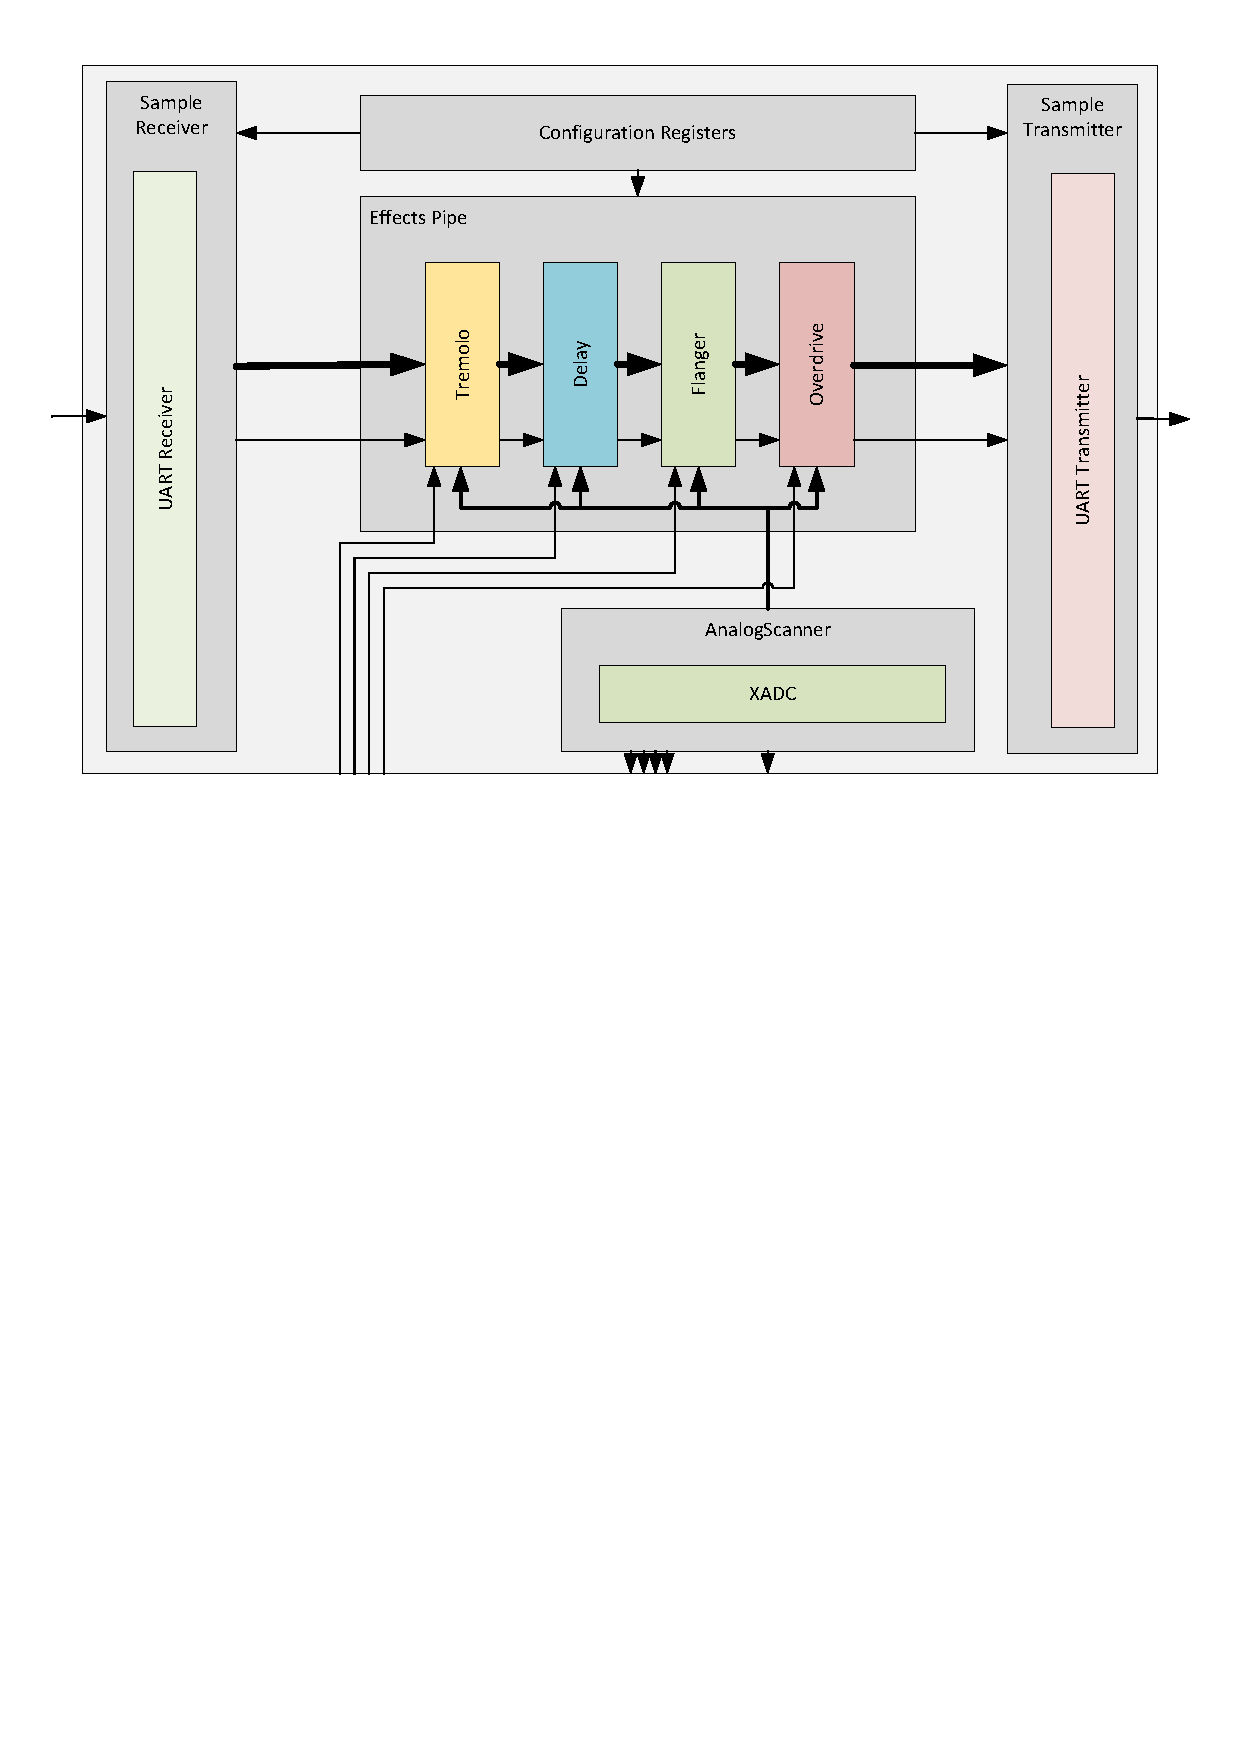
\includegraphics[scale=0.75]{img/diagrams/project_diagram.pdf}
    \captionsetup{format=plain,justification=centering}
    \caption{Struktura implementacyjna projektu}
    \label{fpga-structure}
\end{figure}
\vspace{0.5cm}

Ostatnią - choć nie mniej ważną z~perspektywy projektanta - kwestią wymagającą określenia była struktura samego projektu rozumiana jako podział drzewa plików i~katalogów. Oprogramowanie \textit{Vivado} wykorzystywane na etapie symulacji oraz syntezy nie jest w~opinii autora optymalnym środowiskiem programistycznym\footnote{Vivado jest oczywiście środowiskiem służącym do \textbf{konfiguracji} a~nie programowania układów FPGA. Z~uwagi na brak lepszego terminu postanowiono jednak pozostać przy określeniu \textit{środowisko programistyczne}}. Elementami, które składają się na taki stan rzeczy są m.in. męczący oczy interfejs graficzny oraz brak integracji z~systemami kontroli wersji. Z~tego względu zdecydowano się na wykorzystanie oprogramowania \textit{Visual Studio Code} jako domyślnego narzędzia tworzenia kodu oraz zarządzania projektem. Aby było to możliwe koniecznym stało się zapoznanie się z~odpowiednimi dokumentami (\cite{vivado_design_flow}, \cite{vivado_design_methodology}) udostępnianymi przez firmę Xilinx. Pozwoliło to określić te z~plików generowanych przez \textit{Vivado}, które są konieczne do odtworzenia struktury projektu. Na tej podstawie zdecydowano się na podział przedstawiony na Rys. \ref{project-structure}. Elementami wartymi wyróżnienia są katalogi \textit{src/ip} oraz \textit{workdir}. Pierwszy z~nich przechowuje pliki w~formacie XML opisujące konfigurację wykorzystywanych w~projekcie bloków XADC oraz BRAM (ang. \textit{Block Random Access Memory}), które zostały wyekstrahowane ze struktury projektowej \textit{Vivado}. Drugi stanowi z~kolei miejsce docelowe dla hierarchii plików generowenj przez samo oprogramowanie. Jedynym jej elementem, który włączony został do systemu kontroli wersji jest plik \verb|GuitarMultieffect.xpr| zawierający pełny opis struktury projetktu. Warto zauważyć, że przyjęte podejście do kontroli wersji pozwoli na uruchomienie projektu jedynie przy użyciu aktualnie wykorzystywanej wersji \textit{Vivado} (2020.2).

\vspace{0.5cm}
\begin{figure}[ht]
    \centering
    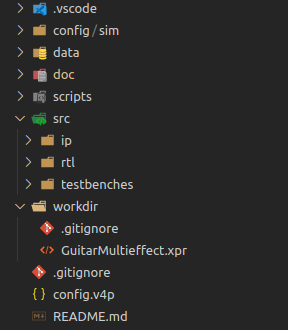
\includegraphics[scale=0.7]{img/source_structure.png}
    \captionsetup{format=plain,justification=centering}
    \caption{Struktura projektowa}
    \label{project-structure}
\end{figure}
\vspace{0.5cm}

\section{Interfejs komunikacyjny}

Budowę interfejsu komunikacyjnego rozpoczęto od zaimplementowania modułów UART. Układ ich wyprowadzeń przedstawiono na Rys. \ref{uart-structure}. Wąskie strzałki symbolizują linie jednobitowe. Strzałki czerwone oraz żółte to linie wielobitowe. Pierwsze z~nich oznaczają, że są port połączony został z~potokiem przetwarzania danych. Z~kolei w~przypadku drugich porty wystawione są poza potok. Konwencja ta została zachowana w~przypadku kolejnych rysunków.

Wejście \verb|clk| to podłączenie do głównego zegara systemowego, natomiast \verb|reset| to asynchroniczny reset układu (aktywny stanem niskim). Wejścia te są uniwersalne dla wszystkich implementowanych modułów. Porty \verb|rate| pozwalają określić szybkość transmisji. Wyrażana jest ona jako ilość cykli zegara systemowego przypadających na jeden znak wysyłany/transmitowany (minus 1). W~przypadku interfejsu odbierającego ustawienie wartości 0~na tym porcie zablokuje odbiór danych\footnote{Stan linii RX testowany jest w~połowie trwania znaku, co wymusza maksymalny stosunek prędkości transmisji do prędkości zegara systemowego na poziomie 1:2}. Oba moduły implementują także linię wyjściową \verb|busy|, która, gdy ustawiona w~stanie wysokim, oznacza, że układ zajęty jest odbiorem/transmisją danych. 

Podsystem odbiorczy udostępnia wyjście odebranych danych \verb|data| oraz oczywiście linię szeregową \verb|rx|. Port \verb|error| reprezentowany jest jako trzybitowa linia typu \verb|record|. Ustawiana jest w~momencie zmiany stanu linii \verb|busy| ze stanu wysokiego na niski i~zawiera flagi błędu odbioru bitu startu, bitów stopu oraz parzystości. Wystąpienie błędu sygnalizowane jest stanem wysokim. Równolegle z~flagami błędów ustawiany jest również port \verb|data|\footnote{W~przypadku wystąpienia błędu odbioru port \textit{data} jest zerowany}. Podsystem nadawczy posiada porty \verb|data| i~\verb|tx| o~znaczeniu analogicznym do przypadku odbiorczego. Udostępnia on także linię \verb|transfer|. Ustawienie jej w~stan wysoki\footnote{Linia aktywna jest \underline{poziomem} wysokim} w~czasie, gdy linia \verb|busy| znajduje się w~stanie niskim, rozpoczyna transmisję danych znajdujących się na wejściu \verb|data|.

\vspace{0.5cm}
\begin{figure}[ht]
    \centering
    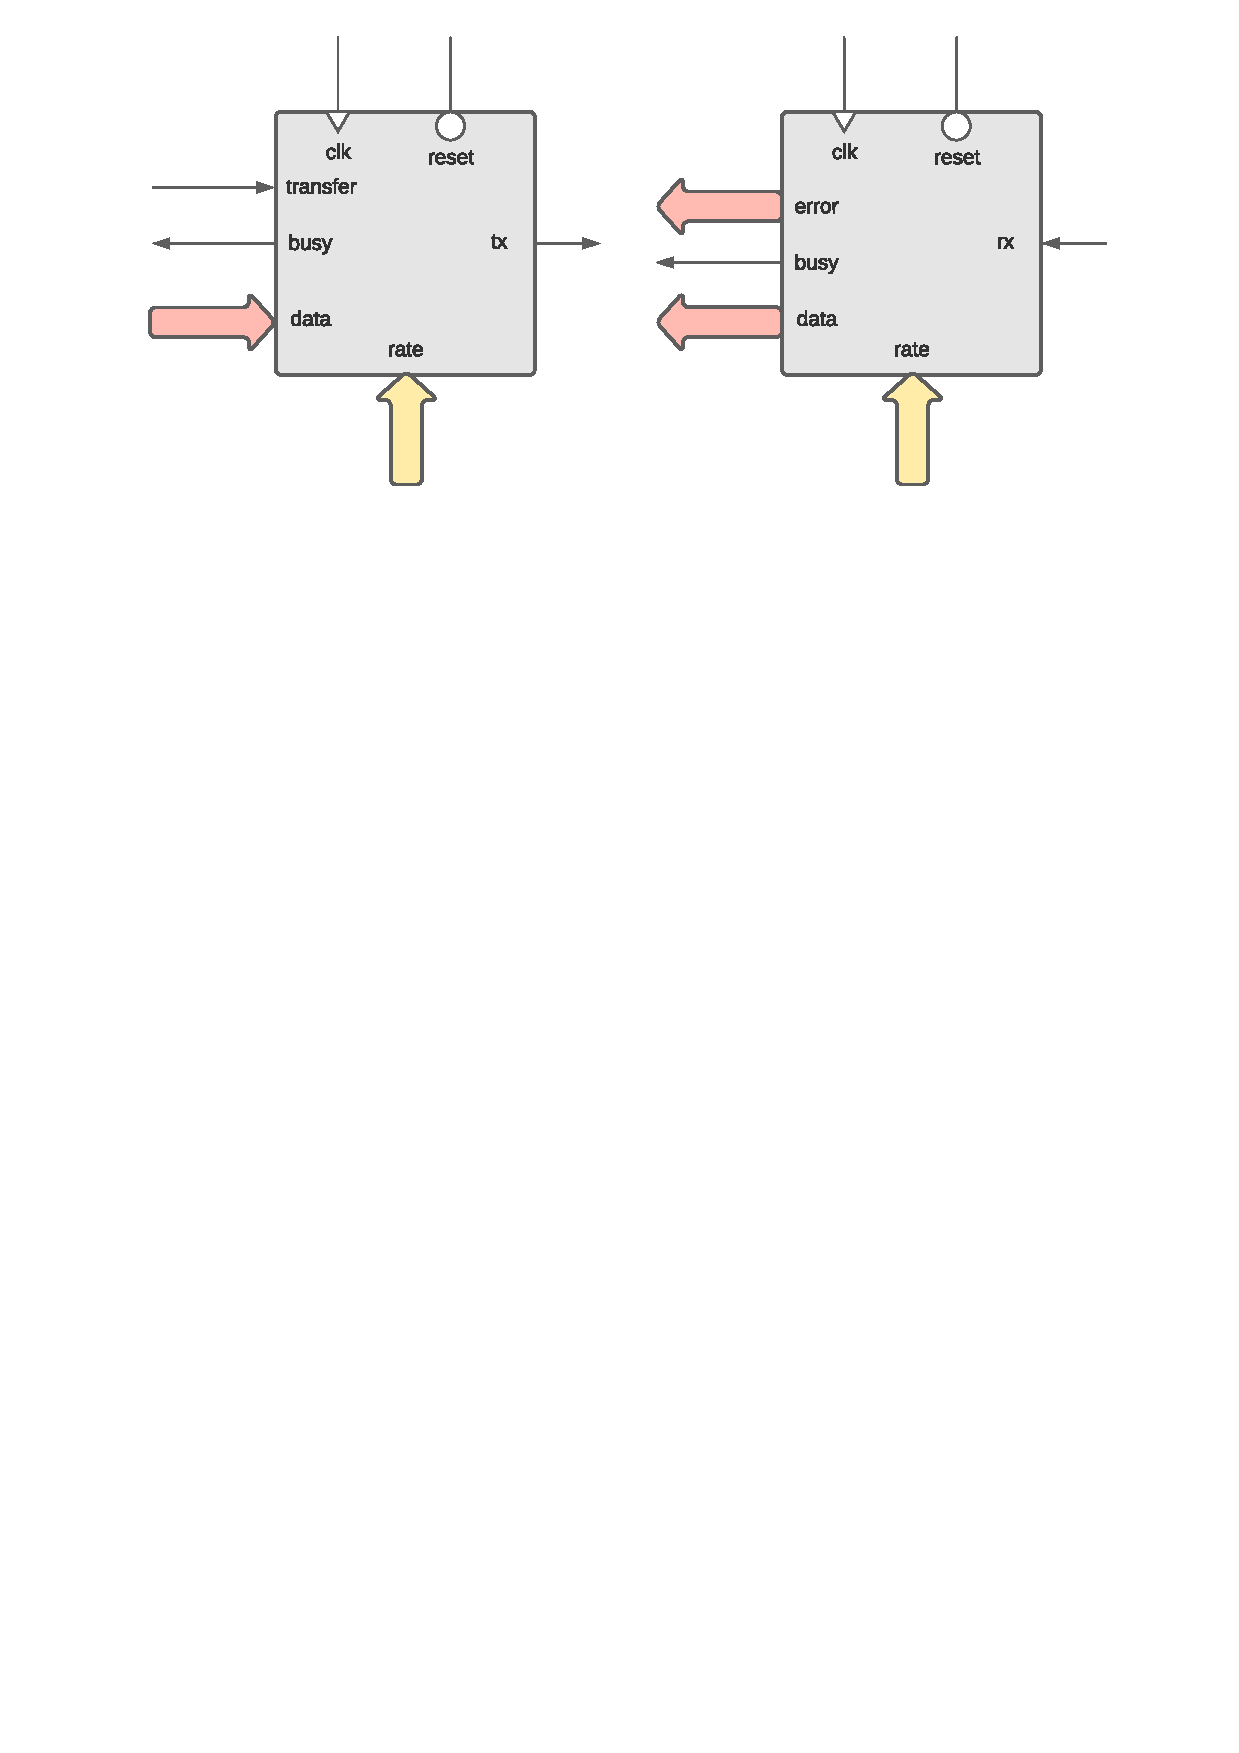
\includegraphics[scale=0.75]{img/diagrams/uart.pdf}
    \captionsetup{format=plain,justification=centering}
    \caption{Struktura wyprowadzeń modułów UART TX orax UART RX}
    \label{uart-structure}
\end{figure}
\vspace{0.5cm}

Struktury \verb|entity| reprezentujące obie podjednostki wyposarzono w~identczny zestaw parametrów (ang. \textit{generic}). Pozwalają one określić szerokość portu \verb|rate| i~format przesyłanych danych (liczbę bitów danych i~stopu oraz rodzaj parzystości). Przy ich pomocy możliwe jest też zanegowanie sygnału transmisyjnego tak, aby bezczynność linii transmisyjnej symbolizowana była stanem wysokim oraz (niezależne) zanegowanie bitów danych. W~projekcie wykorzystane zostały oba rodzaje negacji. 

Obie jednostki zostały zaimplementowane jako synchroniczne automaty skończone o~pięciu stanach. Pierwszy z~nich - \textit{idle} - przyjmowany jest w~momentach bezczynności, tj. gdy moduł oczekuje na wykrycie stanu aktywnego linii odbiorczej lub linii \verb|transfer|. W~momencie zajścia warunków startu automat przechodzi w~stan odbioru/transmisji bitu startu. Przy przejściu tym resetowany jest wewnętrzny licznik długości znaku oraz ustawiana jest linia \verb|busy|. Wartość znajdujące się na wejściu \verb|rate| zapisywana jest w~wewnętrznym buforze. W~przypadku transmisji zapisywana jest także wartość na wejściu \verb|data| a~stan linii \verb|tx| zmieniany jest na aktywny. Rzeczony licznik inkrementowany jest następnie o~jeden w~każdym następnym cyklu zegara systemowego. Moduł odbiorczy oczekuje aż jego wartość dojdzie do połowy zapisanej wartości \verb|rate| (powiększonej o~1), a~następnie próbkuje stan linii \verb|rx| w~celu zweryfikowania stanu bitu startu. Moduł nadawczy czeka natomiast czas dwukrotnie dłuższy. W~przypadku obu jednostek sytuacje te wiążą się z~przejście do kolejnego stanu - odbioru/transmisji bitów danych. Przejście do wszystkich kolejnych stanów (odbioru/nadawania bitów danych, parzystości i~stopu) wiąże się ze zresetowaniem licznika długości trwania znaku. W~przypadku odbioru bitów startu, stopu oraz parzystości odbywa się także ewentualne ustawieniem odpowiedniej flagi błędu w~wewnętrznym buforze. Przejścia do kolejnych stanów wywoływane są osiągnięciem wartości \verb|rate| przez licznik. W~następnym cyklu po odebraniu/nadaniu wszystkich bitów, stan linii \verb|busy| ustawiany jest na niski, a~dane i~flagi błędu (w~przypadku odbioru) kopiowane są z~wewnętrznych buforów na wyjście.

Dla każdego modułu stworzona została symulacja mająca na celu zweryfikowanie poprawności działania. W~jej ramach zostały stworzone procedury biblioteczne realizujące niezależnie funkcjonalność transmisji/odbioru, których kod został oparty na materiałach udostępnionych w~trakcie wykładów. Posiłkowanie się nimi miało na celu eliminację potencjalnych błędów w~procesie weryfikacji.

\vspace{0.5cm}
\begin{figure}[ht]
    \centering
    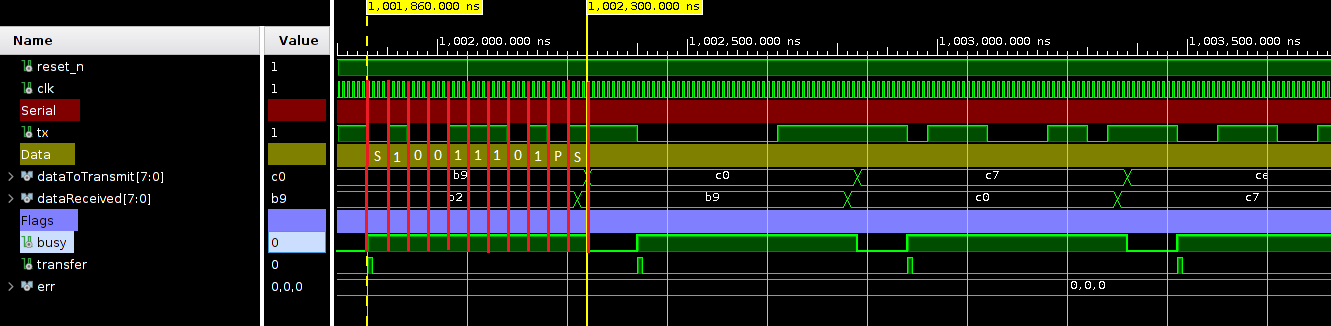
\includegraphics[scale=0.7]{img/sim/communication/uart_tx_sim.png}
    \captionsetup{format=plain,justification=centering}
    \caption{Wycinek sumylacji modułu UART TX}
    \label{sim-uart-tx}
\end{figure}
\vspace{0.5cm}

Symulacje miały charakter całościowy, tj. przetestowane zostały wszystkie kombinacje bitów transmitowanego słowa. Na Rys. \ref{sim-uart-tx} przedstawiono wycinek symulacji modułu TX. Transmitowane dane mają w~tym przypadku format 8E1. Prędkość transmisji to 25MHz natomiast prędkość zegara systemowego to 100MHz. Zastosowano tu zarówno negację sygnału jak i~danych. Pionowe linie w~kolorze czerwonym rozmieszczone zostały w~odstępach czterech cykli zegara systemowego, co odpowiada długości trwania transmitowanego bitu. Przedziadziały oznaczone literami S~odnszą się kolejno do bitu startu oraz bitu stopu. Zgodnie z~oczekiwaniami odpowiadający im stan linii \verb|tx| to odpowiednio niski i~wysoki. Bity danych to kolejno $10011101$. Po odwróceniu ich klejności (słowa transmitowane są w~kolejonści od najmniej do najbardziej znaczącego bitu) otrzymujemy $10111001$. Dane te zapisane w~formacie heksadecymalnym mają postać $0$x$B9$. Identyczna wartość ukazana jest na obrazie symulacji w~wierszu \verb|dataToTransmit|\footnote{Wysyłane słowo były wektorami losowymi z~realizacji rozkładu jednostajnego implementowanego za pomoca funkcji \textit{uniform} biblioteki \textit{math\_real}}, który obrazuje aktualnie transmitowane słowo. Oznacza to, że bity danych zostały nadane poprawnie. Bit parzystości ustawiony jest w~stanie niskim. Biorą pod uwagę nieparzystą liczbę jedynek w~przesyłanym słowie oraz negację sygnału i~danych można stwierdzić, że również ten bit został przesłany poprawnie. Sygnał \verb|dataReceived| jest ustawiany na wartość odebraną przez ww. funkcję biblioteczną. Jak widać, jego wartość zmienia się na oczekiwaną ($0$x$B9$) w~momencie połowy trwania bitu stopu. Na rysunku zaznaczone zestały także momenty ustawienia i~zresetowania stanu linii \verb|busy|. Różnica między nimi opiewa na $440$ ns. Jest to również wartość oczekiwana, ponieważ czas trwania pojedynczego bitu wynosi $40$ ns (cztery takty zegara systemowego) a~sumaryczna liczba transmitowanych bitów to $11$ ($1 + 8 + 1 + 1$). Aby ułatwić weryfikację działania modułu symulacja zostałą zaprojektowana tak, aby w~momencie niezgodności odbieranego znaku z~sygnałem \verb|dataToTransmit| stan bitów linii \verb|dataReceived| ustawiany był na $X$ reprezentowany w~symulacji kolorem czerwonym.

\vspace{0.5cm}
\begin{figure}[ht]
    \centering
    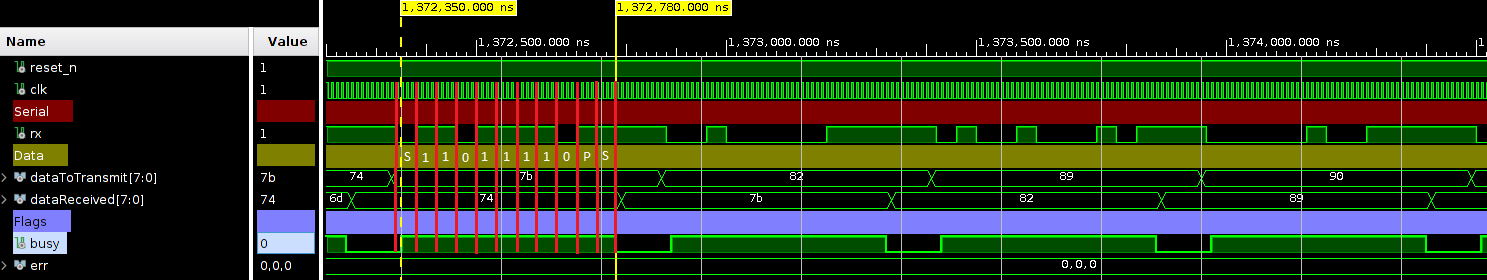
\includegraphics[width=\textwidth]{img/sim/communication/uart_rx_sim.png}
    \captionsetup{format=plain,justification=centering}
    \caption{Wycinek sumylacji modułu UART RX}
    \label{sim-uart-rx}
\end{figure}
\vspace{0.5cm}

Wycinek analogicznej symulacji dla modułu RX (przeprowadzonej przy tych samych parametrach transmisji) został zaprezentowany na Rys. \ref{sim-uart-rx}. Ponowienie analizy przeprowadzonej dla przypadku transmisji pozwala stwierdzić, że również odbiór danych odbywa się prawidłowo. Warto zauważyc, że czas wysoki na linii \verb|rx| trwa o~10 ns krócej, niż w~poprzednim przypadku. Wynika to z~faktu, że automat skończony modułu RX wychodzi ze stanu \textit{idle} dopiero w~momencie odczytania stanu aktywanego na linii odbiorczej\footnote{Po przygotowaniu grafik do sprawozdania zauważono, że moduł RX czeka o~jeden takt zegara za długo na wystawienie odberanych danych (które są gotowe już w~połowie trwania ostatniego bitu stopu). Błąd ten wynikał z~ustawienia niewłaściwego momentu próbkowania bitu startu, który przesuwał pozostałe chwile próbkowania. Został on poprawiony.}.

Przeprowadzone symulacje pozwoliły poprawić początkowe błędy implementacji a~tym samym przejść do kolejnego etapu projektowania interfejsu komunikacyjnego. Było nim stworzenie jednostek akumulujących odbierane i~transmitowane słowa do postaci N-bajto- wych próbek (określanych niżej mianem \textit{SampleTx} i~\textit{SampleRx}). Ich interfejs jest niemal identyczny jak ten przedstawiony na Rys. \ref{uart-structure}. Jedynymi różnicami są szerokość portów \verb|data| oraz brak portów wejściowych \verb|rate|. Szybkość transmisji jest w~ich przypadku ustalana poprzez parametry (\textit{generic}). Wzbogacają one interfejs UART o~dodatkowy N-bajtowy bufor wraz z~multiplexerem o~N~8-bitowych wejściach, którego wyjście połączone jest z~portem \verb|data| wewnętrznej instancji podjednostki UART TX/RX. Układy te pozwalają na odbiór/transmisję próbek w~formacie \textit{little endian} wybranym ze względu na wykorzystanie w~projekcie komputera opartego o~architekturę x86-64. Również w~ich przypadku zaprojektowane zostały symulacje mające na celu sprawdzenie poprawności dekompozycji słów na kolejno wysyłane/odbierane bajty. Filozofia ich działania jest również analogiczna do tej przedstawionej powyżej. Funkcjonalność komplementarna względem testowanego modułu jest implementowana poprzez wykonane wcześniej funkcje biblioteczne wzbogcone o~logikę pozwalającą operować na N-bajtowych słowach. Aktualnie wysyłane dane mogą być obserwowane na symulacji jako sygnał \textit{sampleToTransmit}, natomiast dane odebrane jako sygnał \textit{sampleReceived}. Jeden z~nich ustawiany jest zawsze przez moduł testowany, a~drugi przez proces wywołujący funkcję biblioteczną. Wycinek rzeczonych sumlacji dla przypadku $N=2$ został zaprezentowany na Rys. \ref{sim-sample-trensreceiver}. Niezgodność danych odbieranych z~danymi wysyłanymi lub błąd odbioru sygnalizowane są ponownie ustawieniem bitów sygnału \textit{sampleReceived} w~stan $X$.

\vspace{0.5cm}
\begin{figure}[ht]
    \centering
    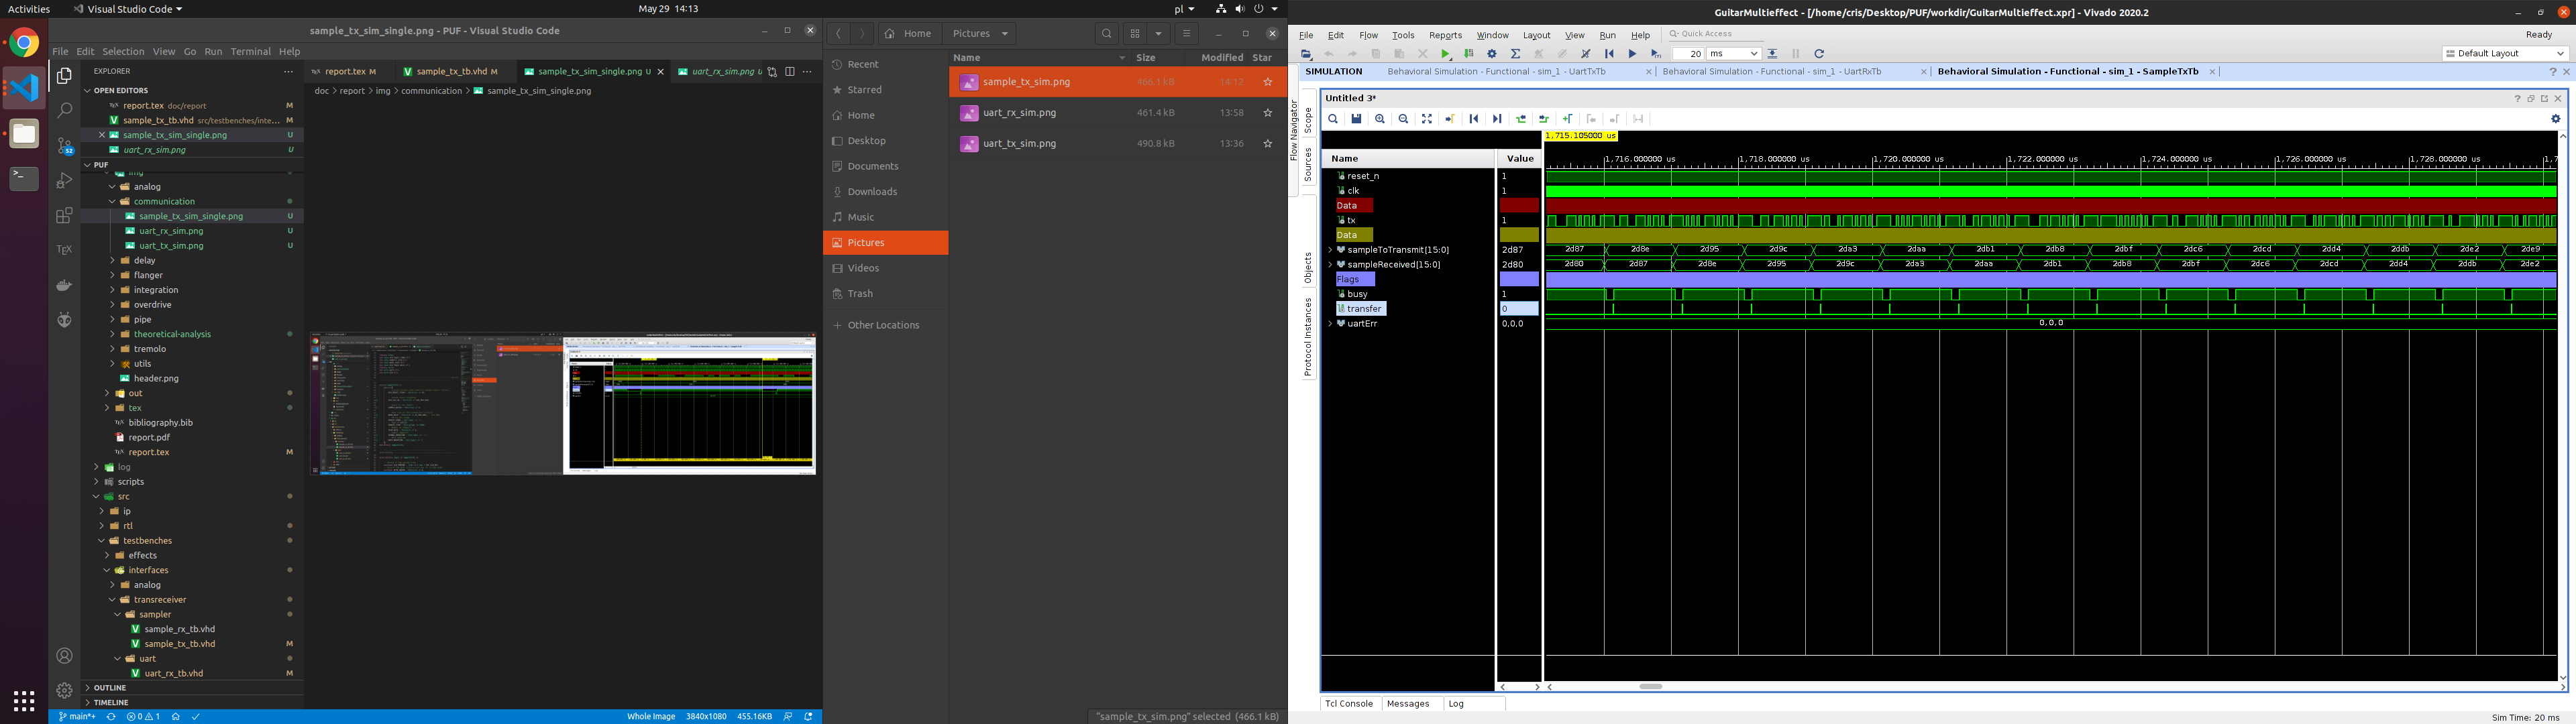
\includegraphics[width=\textwidth]{img/sim/communication/sample_tx_sim_multiple.png}
    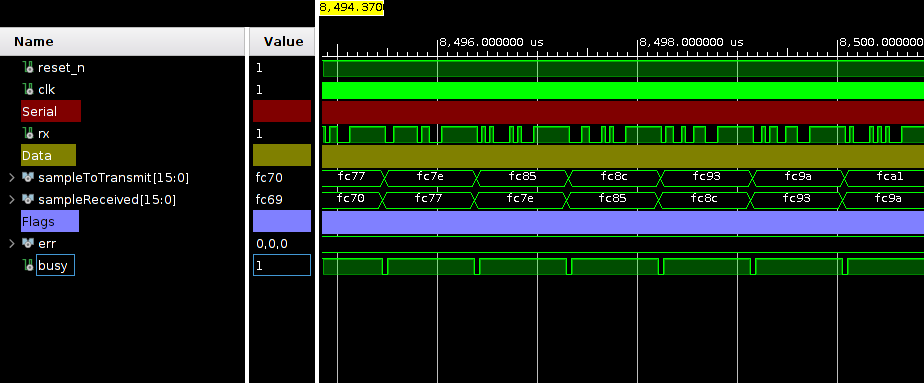
\includegraphics[width=\textwidth]{img/sim/communication/sample_rx_sim_multiple.png}
    \captionsetup{format=plain,justification=centering}
    \caption{Wycinek sumylacji modułów \textit{SampleTx} (u~góry) i~\textit{SampleRx} (u~dołu)}
    \label{sim-sample-trensreceiver}
\end{figure}
\vspace{0.5cm}

\section{Interfejs analogowy}

Drugą z~zaimplementowanych sekcji projektu był interfejs analogwy, który umożliwić miał odczyt wartości napięć na~potencjometrach z~wykorzystaniem zewnętrznego multipleksera analogowego. Zdecydowano się wykorzystać w~tym celu generator IPC (ang. \textit{Intelectual Property Core}) \textit{XADC Wizard} (wersja 3.3). Prace rozpoczęto od zapoznania się zarówno z~dokumentacją modułu ADC dostępnego w~układach FPGA serii sióddmej (\cite{xilinx_adc_series_seven}) jak i~samego generatora (\cite{xilinx_xadc_wizard}). Z~ich pomocą udało się rozszyfrować znaczenie poszczególnych parametrów rdzenia. Zdecydowano się na wykorzystanie interfejsu DRP (ang. \textit{Dynamic Reconfigurable Port}) ze względu na jego relatywną prostotę. XADC został skonfigurowany w~trybie sekwencyjnym (ang. \textit{channel sequencer}) z~manualnym wyzwalanym (ang. \textit{event mode}). Prędkość sygnału zegarowego przyjęto na poziomie 100MHz (zgodnie z~założeniami projektu) natomiast częstotliwość konwersji na poziomie 50KSPS (ang. \textit{KiloSamples Per Second}). Dodatkowo skorzystano z~udostępnianej przez XADC możliwości automatycznego wysterowania linii \textit{select} zewnętrznego multipleksera analogowego. Jako kanał roboczy wybrano \textit{vaux0}, który skonfigurowano w~trybie unipolarnym. Zrezygnowano z~uśredniania wartości próbek w~kanałach oraz dezaktywowano wszystkie alarmy. Ostatnim krokiem było ustawienie odpowiednich wartości w~sekcji \textit{Analog Sim Options} zakładki \textit{Basic}. Wpisano w~niej ścieżkę do zewnętrznęgo pliku zawierającego przebiegi symulowanych wartości analogowych. Jak się później okazało sfinalizowanie tej konfiguracji celem uzyskania możliwości uruchomienia rzeczonej symulacji, wymagało spędzenia dodatkowych kilku godzin na przeglądaniu forum \verb|forum.xilinx.com| celem odszukania informacji brakujących w~dokumentacji.

\vspace{0.5cm}
\begin{figure}[ht]
    \centering
    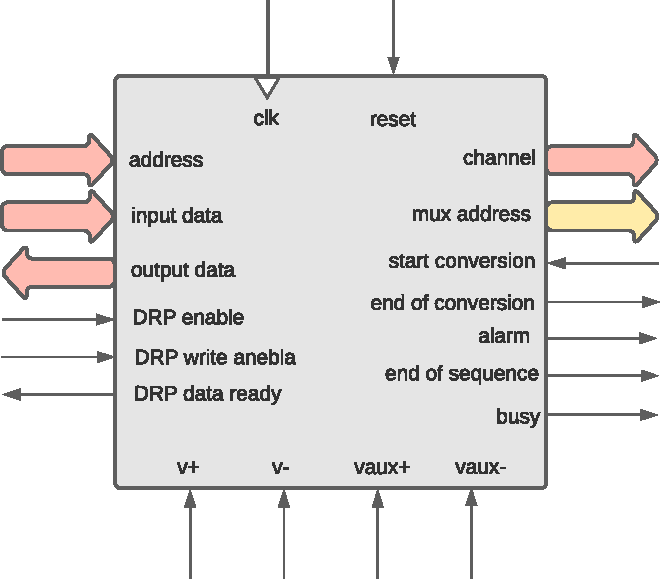
\includegraphics[scale=0.8]{img/diagrams/xadc.pdf}
    \captionsetup{format=plain,justification=centering}
    \caption{Struktura portów wygenerowanego modułu XADC}
    \label{xadc-structure}
\end{figure}
\vspace{0.5cm}

Strukturę wyprowadzeń wygenerowanego bloku funkcjonalnego przedstawiono na Rys. \ref{xadc-structure}. Po lewej stronie przedstawiono sygnały związane z~odczytem i~zapisem wewnętrznych rejestrów modułu. Na dolnej krawędzi znalazły się bipolarne wejścia analogowe. Znaczenie sygnałów zaprezentowanych naprawej krawędzi są następujące:

\begin{itemize}
    \item \textit{channel} - port wyjściowy reprezentujący adres rejestru zawierającego dane z~ostatniego kanału spróbkowanego przez XADC; ustawiany jest na końcu konwersji (niewykorzystany w~projekcie)
    \item \textit{mux address} - linie wysterowujące wejścia \textit{select} zewnętrznego multipleksera analogowego
    \item \textit{start conversion} - linia aktywujące nową konwersję
    \item \textit{end of conversion} - linia ustawiana w~stan wysoki na jeden takt zegara po zakończeniu konwersji
    \item \textit{alarm} i~\textit{end of sequence} - linie alaramu oraz sygnalizacji końca sekwencji aktywne w~stanie wysokim (nieużywane w~projekcie)
    \item \textit{busy} - linia ustawiana w~stan wysoki na czas trwania konwersji
\end{itemize}

Wokół tak przedstawiającej się struktury stworzony został prosty moduł interfejsujący, który automatyzuje cykliczne wyzwalania konwersji oraz odczyt danych z~wewnętrznych rejestrów XADC. Jego struktura została przedstawiona na Rys. \ref{analog-scanner-structure}. Port \verb|data| reprezentowany jest przez tablicę N~wektorów 12-bitowych ($N <= 16$) odzwierciedlających wartości napięcia na kolejnych kanałach multipleksera. W~projekcie wykorzystano dziewięć kanałów (dziewięć potencjometrów), których znaczenie przedstawiono w~dalszej części dokumentu. Na zewnątrz modułu wystawione zostały poza tym wejścia analogowe kanału \textit{vaux0} (oznaczone omyłkowo jako wyjścia) oraz linie \textit{select} dla zewnętrznego multipleksera. Dedykowane wejścia analogowe (\textit{vp/vn}) zostały podłączone na stałe do masy. Parametry (ang.\textit{generic}) modułu pozwalają skonfigurować ilość wykorzystywanych kanałów\footnote{Musi być zgodna z~konfiguracją podaną na etapie generowania XADC} oraz częstotliwość ich próbkowania.
 
\vspace{0.5cm}
\begin{figure}[ht]
    \centering
    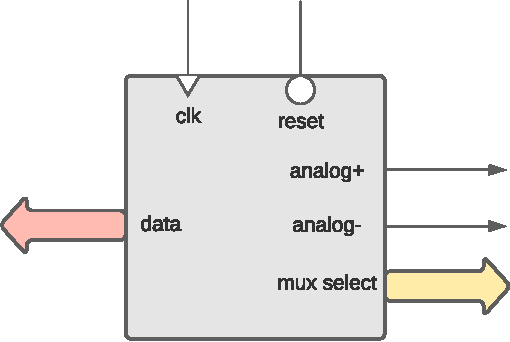
\includegraphics[scale=1.0]{img/diagrams/analog_scanner.pdf}
    \captionsetup{format=plain,justification=centering}
    \caption{Struktura portów bloku skanera kanałów analogowych}
    \label{analog-scanner-structure}
\end{figure}
\vspace{0.5cm}

Zasada działania modułu zasadza się na dwóch synchronicznych procesach. Pierwszy z~nich wyposażony jest w~wewnętrzny licznik, który odmierza takty zegara systemowego między kolejnymi konwersjami. Gdy jego wartość spadnie do zera linia \verb|start conversion| bloku XADC zostaje ustawiona w~stan wysoki na jeden cykl zegara. Równolegle wartość wyjścia \verb|mux address| - powiększona o~wartość $0$x$10$ (adres danych pierwszego kanału pomocniczego \textit{vaux0}) - zostaje przepisana na wejście adresowe interfejsu DRP. Drugi proces implementuje dwustanowy automat skończony. W~pierwszym ze stanów proces oczekuje na pojawienie się logicznej jedynki na linii \verb|end of conversion|. Gdy sytuacja ta zajdzie, linia \verb|DRP enable| również ustawiana jest w~stan wysoki, co rozpoczyna odczyt danych spod adresu znajdującego się na liniach adresowych (ustawianych przez pierwszy proces). Akcja finalizowana jest przejściem do drugiego stanu, w~którym proces pozostaje do wystawienia przez XADC logicznej jedynki na linii \verb|DRP ready| oznaczającej pojawienie się odczytanych danych na procie \verb|output data|. Dane te kopowiane są do odpowiedniego wektora w~tablicy \verb|data| i~proces przechodzi ponownie do stanu pierwszego.

W~celu weryfikacji zaimplementowanego rozwiązania ponownie przygotowano stosowną symulację. Tym razem weryfikacja nie miała charakteru formalnego, tzn. efekty działania testowanego modułu nie były programowo porównywane z~wartościami oczekiwanymi. Ze względu na złożoność implementacji takiego rozwiązania ograniczono się jedynie do weryfikacji jakościowej poprzez manualną analizę zasymulowanych przebiegów. Aby jednak symulacja była możliwa należało najpierw stworzyć odpowiedni plik zawierający przebiegi wartości napięcia na kolejnych kanałach ADC. Generację takowego pliku zautomatyzowano za pomocą prostego skryptu języka Python, który pozwala zdefiniować długość trwania generowanych sygnałów, ich przebieg oraz częstotliwość ``próbkowania''. Z~jego pomocą wygenerowano sinusoidalny przebieg napięcia na kanale \textit{vauxp0} ustawiając jednocześnie pozostałe kanały na wartość~$0$. Fragment symulacji obrazuje Rys. \ref{sim-analog-scanner}. Przyjęto w~niej częstotliwość konwersji na maksymalnym poziomie 50KSPS. Jak widać wektory tabeli \textit{channels\_out} (podłączej do portu wyjściowego \verb|data| skanera) są aktualizowane w~zakładany sposób. Dla lepszego zobrazowania sposobu działania układu rysunek ukazuje także bezpośrednie przebiegi niektórych portów modułu XADC. 

\vspace{0.5cm}
\begin{figure}[ht]
    \centering
    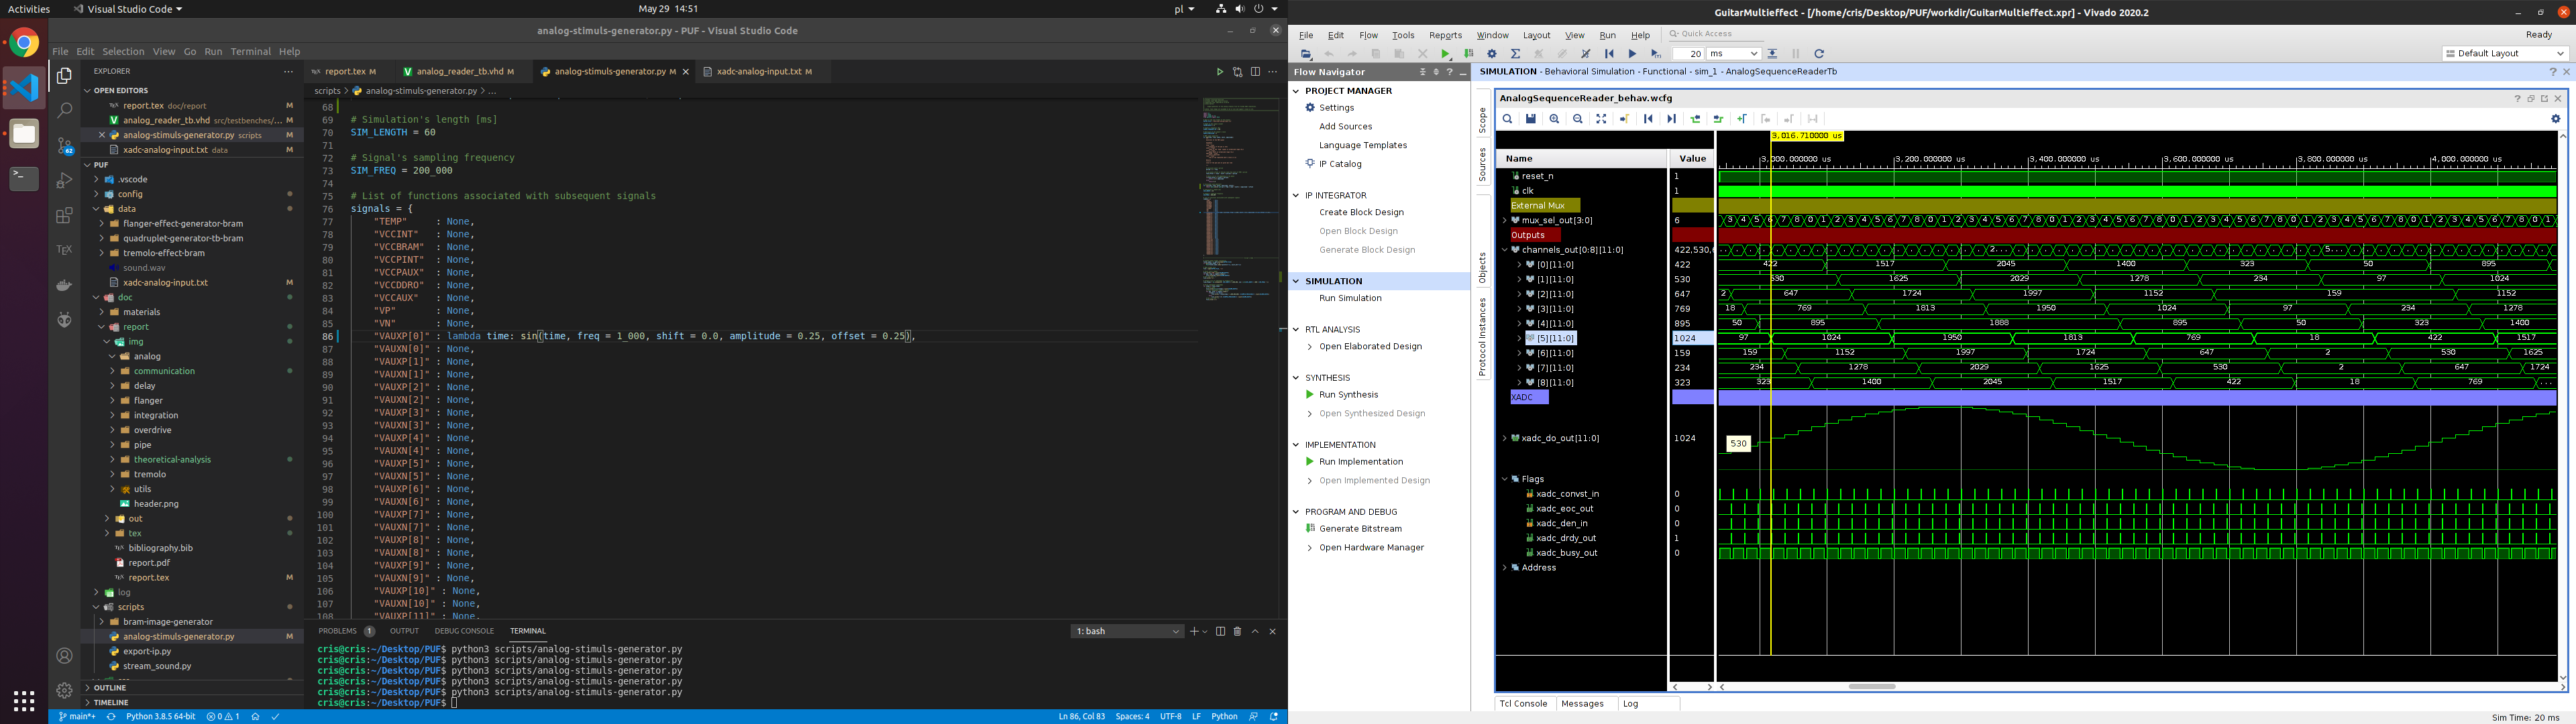
\includegraphics[width=\textwidth]{img/sim/analog_scanner_sim.png}
    \captionsetup{format=plain,justification=centering}
    \caption{Fragment symulacji bloku skanera analogowego}
    \label{sim-analog-scanner}
\end{figure}
\vspace{0.5cm}

\section{Efekt \textit{overdrive}}

Pierwszym z~zaimplementowanych efektów dźwiękowych był tzw. przester (ang. \textit{overdrive}). Został on wybrany ze względu na możliwość relatywnie prostej realizacji. Schemat jego wyprowadzeń został przedstawiony na Rys. \ref{overdrive-structure}. Inkorporuje on siedem portów uniwersalnych dla wszystkich realizowanych efektów. Pierwsze dwa to \verb|clk| i~\verb|reset| opisane przy okazji omawiania modułów UART. Porty \verb|input data| oraz \verb|output data| stanowią wejście i~wyjście danych z~efektu\footnote{Dane traktowane są jako N-bitowe liczby w~formacie U2}. Przepisanie danych wejściowych do wewnętrznego bufora odbywa się po pojawieniu się stanu wysokiego na wejściu \verb|valid in|. Z~kolei na wyjściu \verb|valid out| logiczna jedynka ustawiana jest w~momencie wystawienia przetworzonych danych na czas trwania jednego cyklu zegarowego. Gdy wejście \verb|enable| znajduje się w~stanie niskim dane przepisywane są synchronicznie z~wejścia na wyjście bez wprowadzania zmian. Tak zaprojektowany interfejs pozwala - zgodnie z~założeniami - łączyć poszczególne efekty w~dowolnej koleności bez potrzeby ingerowania w~ich wewnętrzną strukturę.

\vspace{0.5cm}
\begin{figure}[ht]
    \centering
    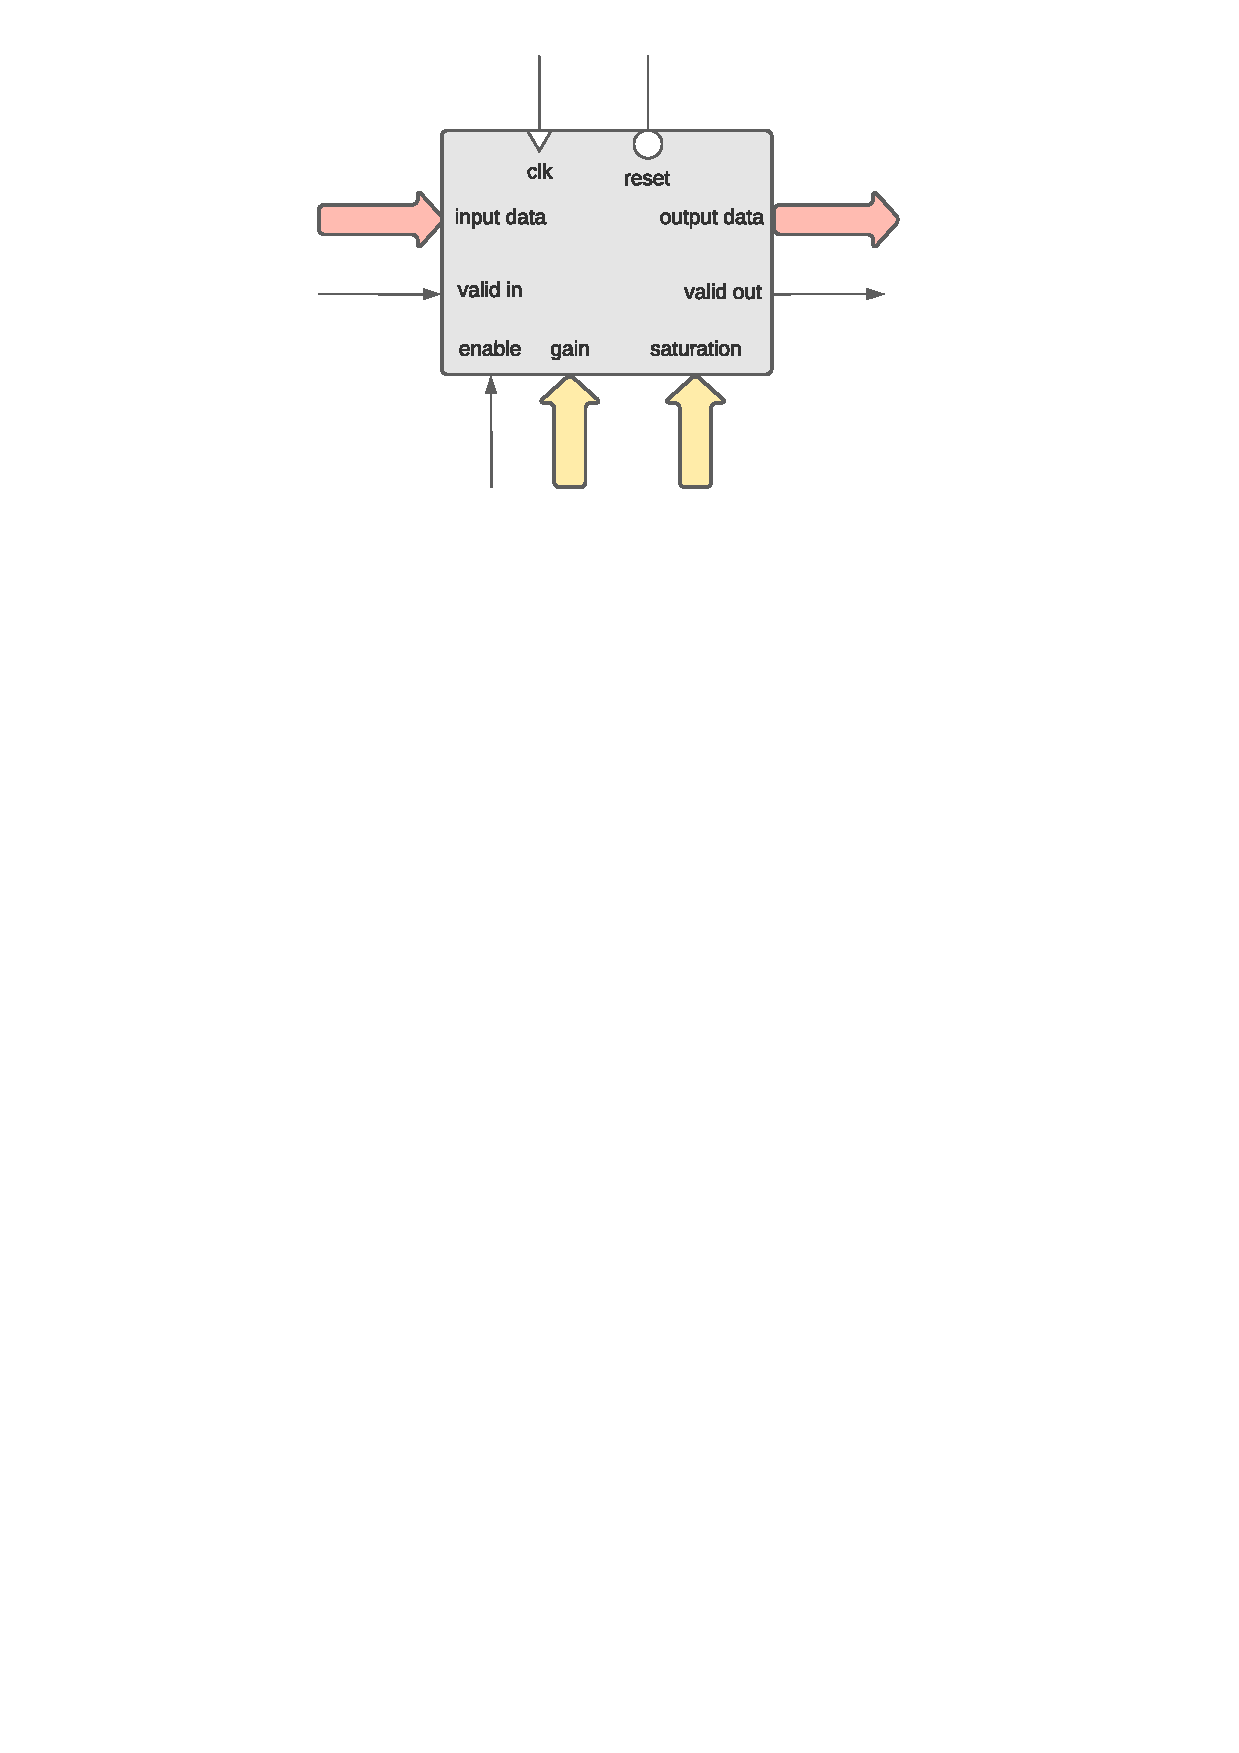
\includegraphics[scale=0.75]{img/diagrams/overdrive.pdf}
    \captionsetup{format=plain,justification=centering}
    \caption{Struktura wyprowadzeń bloku \textit{overdrive}}
    \label{overdrive-structure}
\end{figure}
\vspace{0.5cm}

Dwa dodatkowe porty wejściowe - \verb|gain| oraz \verb|saturation| - pozwalają dostosowywać parametry charakterstyczne filtra. Pierwszy z~nich określa czynnik przez jaki mnożona jest próbka wejściowa. Z~kolei drógi określa poziom obustronnego nasycenia wyniku mnożenia przed wystawieniem go na wyjście. Oba parametry traktowane są jako liczby bez znaku. Parametry modułu (\textit{generic}) pozwalają określić szerokość przetwarzanych próbek oraz wejścia \verb|gain|. Szerokość wejścia \verb|saturation| jest zawsze o~jeden bit mniejsza od szerokości próbek i~determinuje ograniczenie na \underline{wartość bezwzględną} próbki wyjściowej. Opcjonalnie możliwe jest też określenie przesunięcia bitowego (w~prawo) wyniku mnożenia przed podaniem go do bloku nasycenia. Pozwala to przeskalować efektywny zakres parametru \verb|gain| do obszaru wartości niecałkowitych.

Zasada działania modułu jest stosunkowo prosta. Po wykryciu stanu wysokiego na linii \verb|valid in| dane wejściowe, oraz parametry \verb|gain| i~\verb|saturation| przepisywane są do wewnętrznych buforów. Zawartość bufora danych i~wzmocnienia jest asynchronicznie mnożona (z~nasyceniem w~zakresie reprezentacji\footnote{W~ramach prac nad modułem \textit{overdrive} stworzona zostały cztery pomniejsze moduły DSP implementujące operacje dodawania i~mnożenia z~nasyceniem liczb z~i~bez znaku o~arbitralnej długości. Zostały one wykorzystane przy implementacji kolejnych efektów.}). W~następnym takcie zegara wynik mnożenia - opcjonalnie przesunięty o~skonfigurowaną liczbę bitów - zostaje nasycony w~granicach określonych przez bufor \verb|saturation| i~wystawiony na wyjście układu. Czas przetwarzania próbki wynosi \textbf{1~cyklu}. Jeżeli wejście \verb|enable| znajduje się w~stanie niskim, czas ten spada oczywiście do zera. 

Tak jak w~przypadku interfejsu analogowego stworzona została symulacja, której celem miała być jakościowa ocena pracy układu. Jej fragment ukazuje Rys. \ref{sim-overdrive}. Do testów wykorzystano falę sinusoidalną o~częstotliwości 440Hz reprezentowaną za pomoca próbek 16-bitowych. Szerokość wejścia \verb|gain| określono na $12$ bitów, przy czym wyjście z~układu mnożącego przesówane było o~$10$ bitów. Pozwala to na ustawianie wzmocnienia sygnału w~zakresie $[0,4)$. Jak widać na ukazanych przebiegach, włączenie modułu skutkuje wystąpieniem charakterystycznego ``przycinania'' próbek wejściowych.

\vspace{0.5cm}
\begin{figure}[ht]
    \centering
    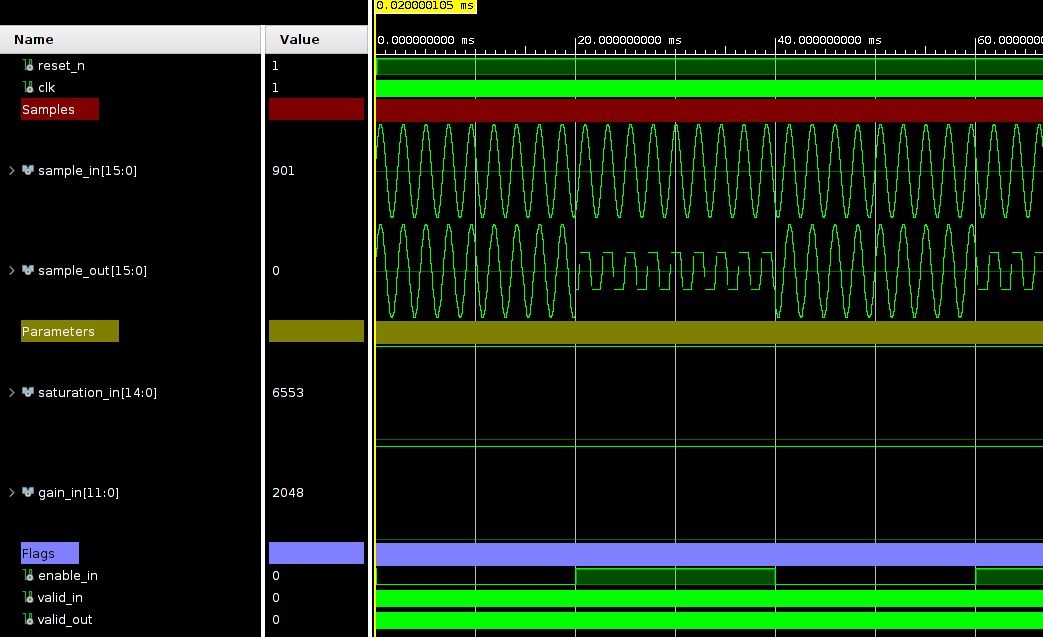
\includegraphics[width=\textwidth]{img/sim/overdrive_sim.png}
    \captionsetup{format=plain,justification=centering}
    \caption{Fragment symulacji działania efektu \textit{overdrive}}
    \label{sim-overdrive}
\end{figure}
\vspace{0.5cm}
\section{Efekt tremolo}

Następnym pod względem skompilikowania, a~co za tym idzie pod względem kolejności implementacji, był efekt tremolo. Jak nakreślono w~części pierwszej, polega on na modulacji sygnału wejściowego wolnozmiennym sygnałem okresowym(LFO, ang. \textit{Low Frequency Oscilator}). Schemat wyprowadzeń gotowego efektu przedstawia Rys. \ref{tremolo-structure}. Podobnie jak w~przypadku poprzedniego efektu mamy tu do czynienia z~dwoma parametrami: \verb|depth| oraz \verb|period|. Pierwszy z~nich - głębokość - określa siłę efektu modulacji. Jego nazwa wzięła się od formuły służącej do obliczania wartości próbki zmodulowanej: 

\begin{equation}
    y[t] = x[t] \times (1 - d \times m[t])
\end{equation}

\noindent
gdzie $y[t]$ - wartość wyjściowa, $x[t]$ - wartość wejściowa, $m[t]$ - wartość fali modulującej (w~zakresie $[0,1]$), $d$ współczynnik głębokości (w~zakresie $[0,1]$). Jak widać, zwiększenie wartości $d$ powoduje, że efektywny zakres modulacji zbliża się do poziomu $0$. Drugi parametr - okres - określa ilość taktów zegara systemowego przypadających na pojedynczą próbkę fali modulującej. Jest to dość dziwna wartość parametryzująca, jednak pozwala na elastyczne dostosowywanie zakresu częstotliwości modulujących oferowanych przez efekt. Parametry układu pozwalają określić szerokość wejść parametryzujących, portów danych danych oraz rozdzielczość próbek sygnału wolnozmiennego.

Implementacja jednostki umożliwia wykorzystanie jednej z~dwóch funkcji modulujących: sinus oraz falę trójkątną. Generatory obu z~nich zostały zrealizowane jako niezależne bloki funkcjonalne. Generator funkcji sinus zaimplementowano przy użyciu modułów RAM obecnych w~FPGA (\cite{xilinx_memory_seven}). Do ich zinterfejsowania wykorzystano IPC \textit{Block Memory} w~wesji 8.3 (\cite{xilinx_bram_wizard}). Pamięć skonfigurowano w~trybie \textit{Native} stosując pojedynczy bufor wyjściowy\footnote{Wiązało się to ze~zwiększeniem opóźnień operacji odczytu do dwóch cykli.}. Jej celem jest przechowywanie N-bitowych próbek z~pierwszej ćwiartki okresu funkcji sinus. Pozostała część fali generowana jest przez moduł z~wykorzystaniem odpowiednich symetrii. Określenie zawartości pamięci odbywa się na etapie konfiguracji IPC. Wykorzystywane są w~tym celu pliki w~formacie COE (skrót od ang. \textit{coefficient}. Ich generacja odbywa się dwuetapowo). W~pierszym kroku generowany jest plik tekstowy zawierający kolejne próbki fali w~formacie heksadecymalnym. Skrypt ten został stworzony w~ramach projektu. Następnie plik wynikowy jest przekazywany do skryptu zaczerpiniętego z~\cite{coe_generator}, który przetwarza dane wejściowe do porządanego formatu.

\vspace{0.5cm}
\begin{figure}[ht]
    \centering
    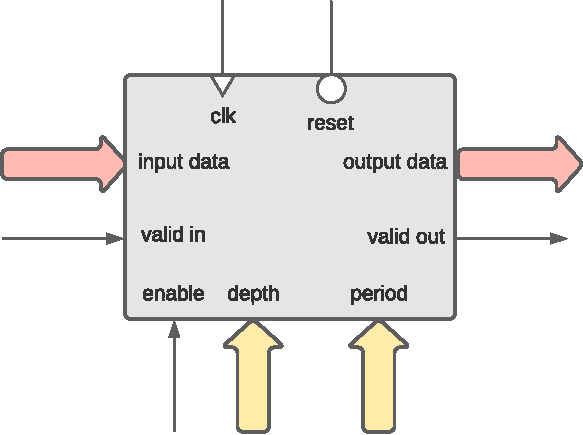
\includegraphics[scale=0.75]{img/diagrams/tremolo.pdf}
    \captionsetup{format=plain,justification=centering}
    \caption{Struktura wyprowadzeń bloku tremolo}
    \label{tremolo-structure}
\end{figure}
\vspace{0.5cm}

Implementacja generatora fali trójkątnej była dużo prostsza i~sprowadzała się do realizacji dwukierunkowego licznika. Gdy oba generatory zostały wdrożone\footnote{...oraz przetestowane z~wykorzystaniem dedykowanyc symulacjii}, realizacja efektu stała się formalnością. Jego architektura podzielona została na dwa procesy. Pierwszy z~nich odpowiada za generowanie fali modulującej. W~każdym takcie zegara wartość wewnętrznego licznika porównywana jest z~wartością na wejściu \verb|period|. Jeżeli są one równe, generowana jest następna próbka. W~przeciwnym wypadku licznik jest inkementowany. Drugi z~procesów monitoruje wejście \verb|valid in|. Gdy jego stan zostanie ustawiony na wysoki, próbka wejściowa oraz parametr \textit{depth} zostają przepisane do wewnętrznych buforów. Obliczenie wartości próbki wynikowej zgodnie z~ww. wzorem zachodzi asynchronicznie. Jako że iloczyn $d \times m[t]$ nie zawiera się w~przedziale $[0,1]$ koniecznym staje się przesunięcie wyniku tej operacji w~prawo o~liczbę bitów będącą sumą szerokości próbki generatora i~szerokości wejścia \verb|depth|. W~następnym po zapisaniu buforów przetworzona próbka zostaje wystawiona na wyjście układu. Zastosowany rozdział obsługi LFO oraz przetwarzania sygnału wyjściowego pozwoliło uniezależnić opóźnienie całego modułu od opóźnienia zastosowanego generatora. W~ten sposób udało się uzyskać opóźnienie na poziomie \textbf{1~cyklu}.

Wycinek symulacji przeprowadzonych dla efektu tremolo został przedstawiony na Rys. \ref{sim-tremolo}. Sygnał wejściowy to ponownie fala sinus o~częstotliwości $440$Hz. Wartość współczynnika \verb|period| dobrana została tak, aby uzyskać częstotliwość modulacji na poziomie $70$Hz. Współczynnik głębokości ustawiono na najwyższą wartość. Zastosowano modulację z~wykorzystaniem 8-bitowej fali trójkątnej. Analogiczne symulacje przeprowadzone zostały również dla drugiego typu modulacji. W~obu przypadkach układ wydaje się działać prawidłowo. 

\vspace{0.5cm}
\begin{figure}[ht]
    \centering
    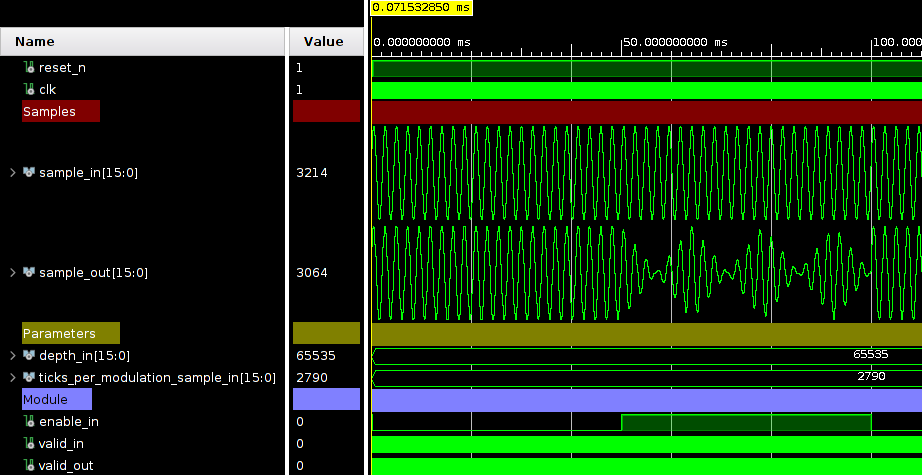
\includegraphics[width=\textwidth]{img/sim/tremolo_sim.png}
    \captionsetup{format=plain,justification=centering}
    \caption{Fragment symulacji działania efektu tremolo}
    \label{sim-tremolo}
\end{figure}
\vspace{0.5cm}
\section{Efekt pogłosu}

Doświadczenia w~wykorzystywaniu bloków BRAM nabyte w~czasie implementacji generatora funkcji sinus pozwoliły na sprawną realizację kolejnego z~zaplanowanych efektów - pogłosu. Prace nad nim rozpoczęto od zaimplementowania parametryzowalneog \textbf{modułu opóźnienia}, ktory miał zostać użyty również w~przypadku kolejnego efektu. Zasada jego działania jest stosunkowo prosta i~zasadza się na sekwencyjnym zapisie próbek wejściowych w~pamięci RAM - traktowanej jako bufor kołowy - oraz odczycie próbek spod adresu będącego wynikiem odejmowania adresu aktualnie zapisywanej próbki i~parametru zewnętrznego (stopnia opóźnienia). Blok ten implementuje wejście i~wyjście danych oraz długość opóźnienia, wyjście \verb|busy| informujące o~możliwości odebrania opóźnionej próbki z~wyjścia oraz wejście \verb |enable| umożlwiające rozpoczęcie przetwarzenia próbki wejściowej. Jego strukturę zewnętrzną przedstawiono na Rys. \ref{delay-line-structure}.

\vspace{0.5cm}
\begin{figure}[ht]
    \centering
    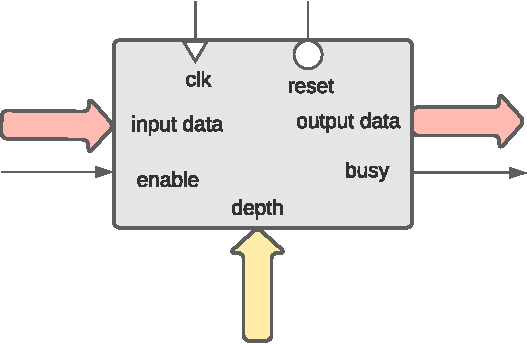
\includegraphics[scale=0.75]{img/diagrams/delay_line.pdf}
    \captionsetup{format=plain,justification=centering}
    \caption{Struktura wyprowadzeń modułu opóźniającego}
    \label{delay-line-structure}
\end{figure}
\vspace{0.5cm}

Porty bloku efektu zostały z~kolei ukazane na Rys. \ref{delay-structure}. Posiada dwa wejścia określające kolejno głębokość echa (\verb|depth|) oraz jego siłę (\verb|delay|). Pierwszy parametr interpretowany jest jako opóźnienie próbki odczytywanej z~bloku opóźniającego. Z~kolei drugi traktowany jest jako liczba z~zakresu $[0,5)$ przez którą mnożone jest wyjście bloku opóźniającego przed zsumowaniem go z~aktualną próbką wejściową.

\vspace{0.5cm}
\begin{figure}[ht]
    \centering
    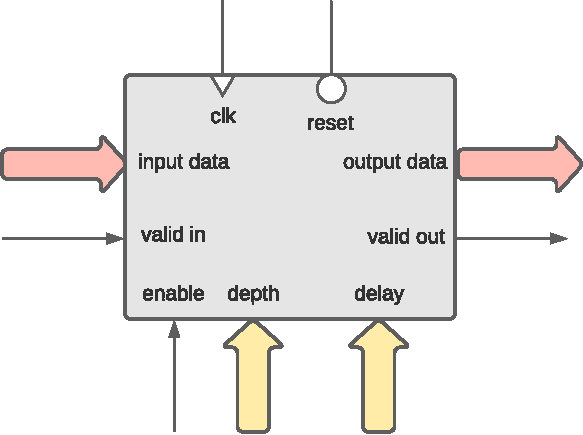
\includegraphics[scale=0.75]{img/diagrams/delay.pdf}
    \captionsetup{format=plain,justification=centering}
    \caption{Struktura wyprowadzeń bloku \textit{delay}}
    \label{delay-structure}
\end{figure}
\vspace{0.5cm}

Dzięki wydzieleniu większego elementu efektu w~postaci odrębnego bloku funkcjonalnego, proces dalszej jego realizacji był znacznie ułatwiony. Logika moduły sprowadzona została do dwustanowego automat skońćzony. W~stanie \textit{idle} moduł oczekuje na pojawienie się jedynki logicznej na porcie \verb|enable|. Gdy zostanie ona wykryta, wartości na z~portów danych oraz parametrów są przepisywane do wewnętrznych buforów. Jednocześnie stan linii \verb|enable| modułu opóźniającego oraz wyjścia \verb|busy| efektu ustawiany jest na wysoki. Wejście danych podłączone jest na stałe do bufora \textbf{wyjściowego} efektu co oznacza, że w~pamięci BRAM zapisana zostanie próbka wynikowa \textbf{poprzedniego cyklu przetwarzania}. Po uruchomieniu bloku opóźnienia moduł przechodzi do stanu oczekiwania na wynik. Jego pojawienie się na wyjściu bloku sygnalizowane jest przez opadające zbocze portu \verb|busy|. W~momencie jego wykrycia aktualizowany jest stan bufora danych wyjściowych. W~zależności, czy zbuforowana wartość parametru \verb|depth| jest zerowa czy nie, na wyjście trafia nieprzetworzona wersja danych wyjściowych lub wynik (asynchronicznego) dodawania zawartości bufora wejściowego z~iloczynem wyjścia z~bloku opóźniającego z~wartością bufora \verb|delay|\footnote{Wynik iloczynu jest przesunięty w~prawo o~liczbę bitów o~jeden większą niż szerokość wejścia \textit{depth}}. Dodawanie odbywa się z~nasyceniem w~zakresie reprezentacji. Warto dodać, że blok opóźniający posiada (opcjonalną) funkcję miękkiego startu, która ogranicza wartość realizowanego opóźnienia do ilości próbek zapisanych w~pamięci BRAM od ostatneigo resetu. Ma ona na celu zredukowanie potencjalnych zniekształceń sygnału na początku działania efektów wynikajacych z~wykorzystania niezainicjalizowanych komórek pamięci jako właściwych danych.

Do realizacji bloku opóźniającego w~przypadku efektu \textit{delay} wykorzystano 21 bloków RAM, których łączna pojemność umożliwi przechowanie do $45056$ 16-bitowych próbek danych. Dla częstotliwości próbkowania na poziomie 44100Hz oznacza to możliwość osiągnięcia opóźnień rzędu jednej sekundy. Ze względu na zastosowanie bufora na wyjściu bloku BRAM opóźnienie efektu wynosi \textbf{4~cykle}. Analogicznie do przypadku poprzednich efektów celem weryfikacji poprawności działania modułu skonstruowany został projekt symulacji umożliwiający realizację różnych scenariuszy testowych. Rys. \ref{sim-delay} przedstawia fragment symulacji, w~którym wartość opóźnienia została ustalona na poziomie 255 próbek, natomiast jego siła miała wartość maksymalną ($0.5$). Sygnał wejściowy to ponownie fala sinusoidalna o~częstotliwości $440$Hz próbkowana z~częstotliwośicą $44100$Hz. Jak widać włączenie efektu nie powoduje natychmiastowej zmiany charakteru sygnału. Zmiana ta następuje po czasie około $5.8$ ms. Zgadza się to z~przewidywaniami teoretycznymi ($1s / 44100 \times 255 \approx 5.8 ms$). Ponadto symulacja ukazuje zmniejszenie amplitudy sygnału po dodaniu do niego składnika opóźnionego. To również zgadza się z~przewidywaniami. Opóźnienie $255$ próbek odpowiada niecałym $2.5$ okresom sygnału wejściowego. Oznacza to, że znaki próbki wejściowej i~opóźnionej są względem siebie odwrócone, co powoduje efektywne zredukowanie amplitudy fali wyjściowej.

\vspace{0.5cm}
\begin{figure}[ht]
    \centering
    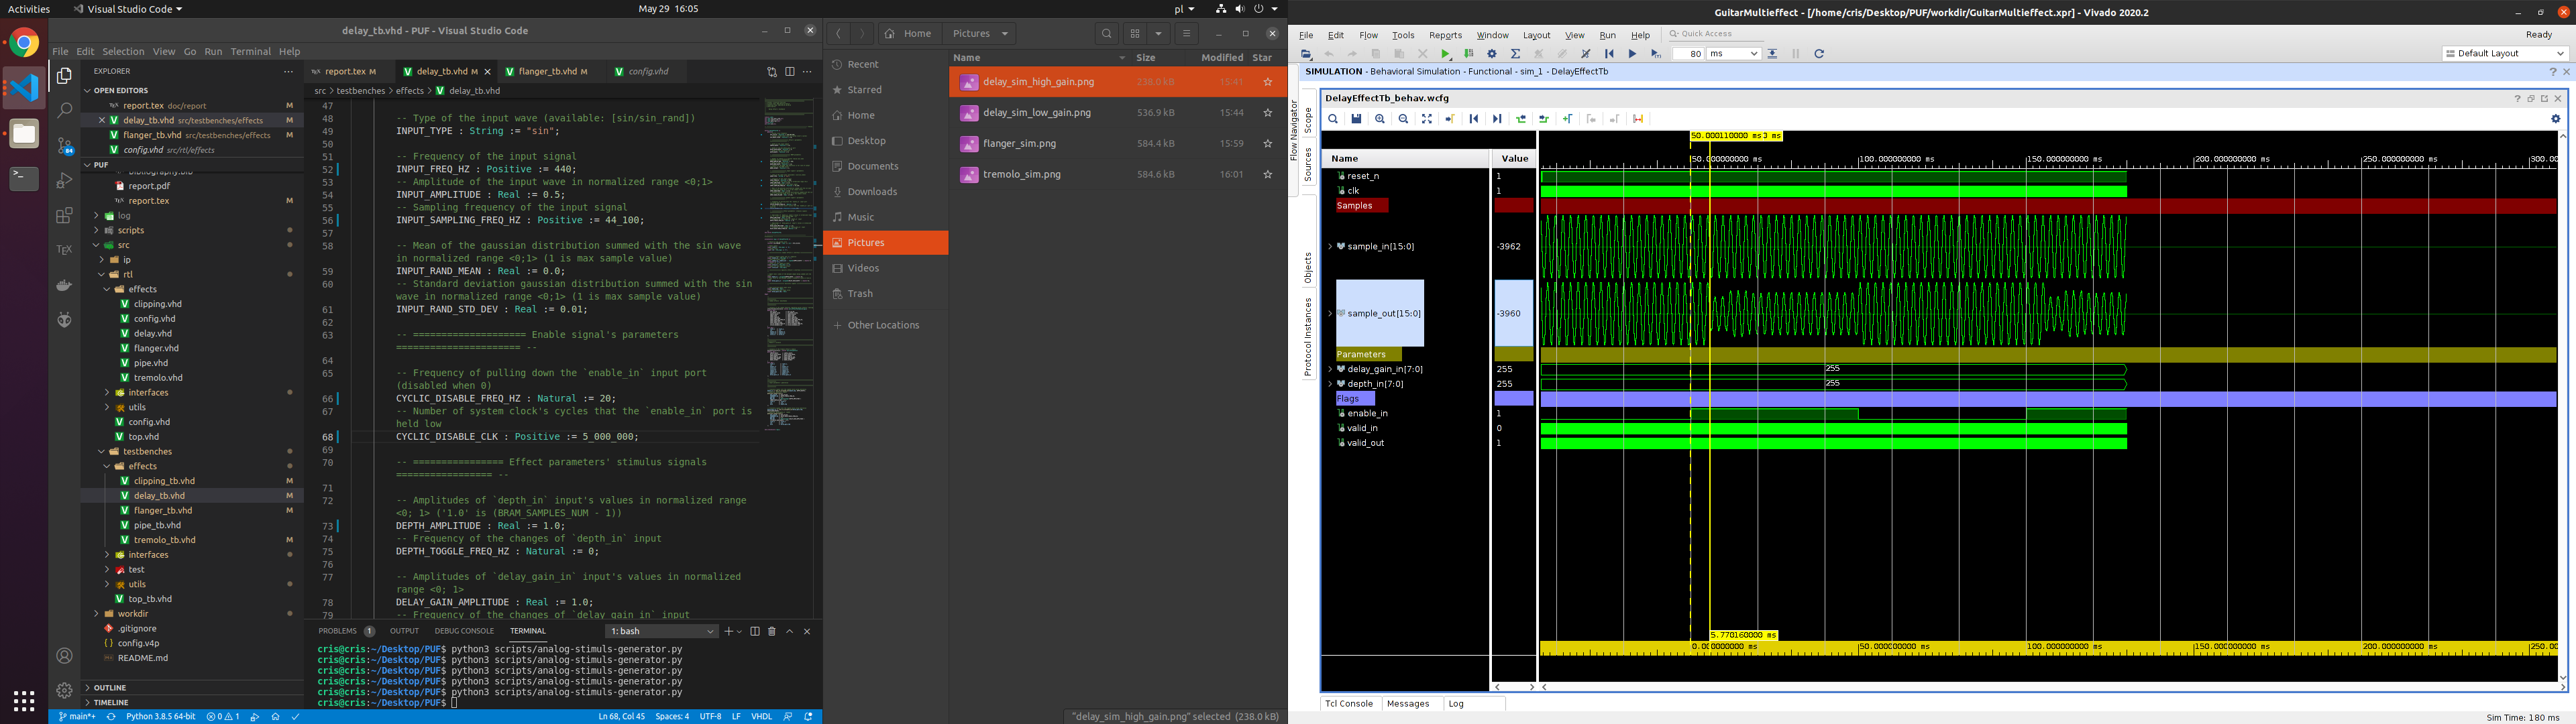
\includegraphics[width=\textwidth]{img/sim/delay_sim_high_gain.png}
    \captionsetup{format=plain,justification=centering}
    \caption{Fragment symulacji działania efektu \textit{delay}}
    \label{sim-delay}
\end{figure}
\vspace{0.5cm}
\section{Efekt \textit{flanger}}



\vspace{0.5cm}
\begin{figure}[ht]
    \centering
    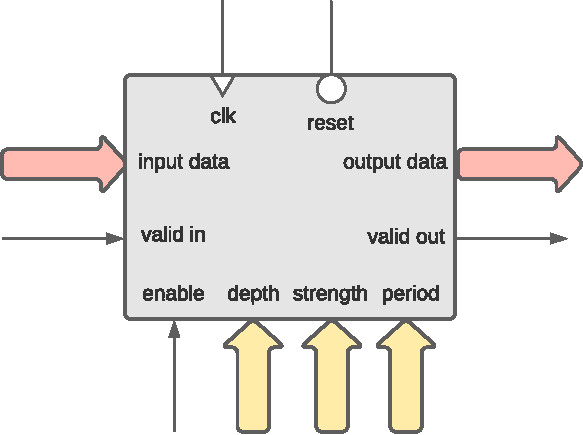
\includegraphics[scale=0.75]{img/diagrams/flanger.pdf}
    \captionsetup{format=plain,justification=centering}
    \caption{Struktura wyprowadzeń bloku \textit{flanger}}
    \label{flanger-structure}
\end{figure}
\vspace{0.5cm}

\vspace{0.5cm}
\begin{figure}[ht]
    \centering
    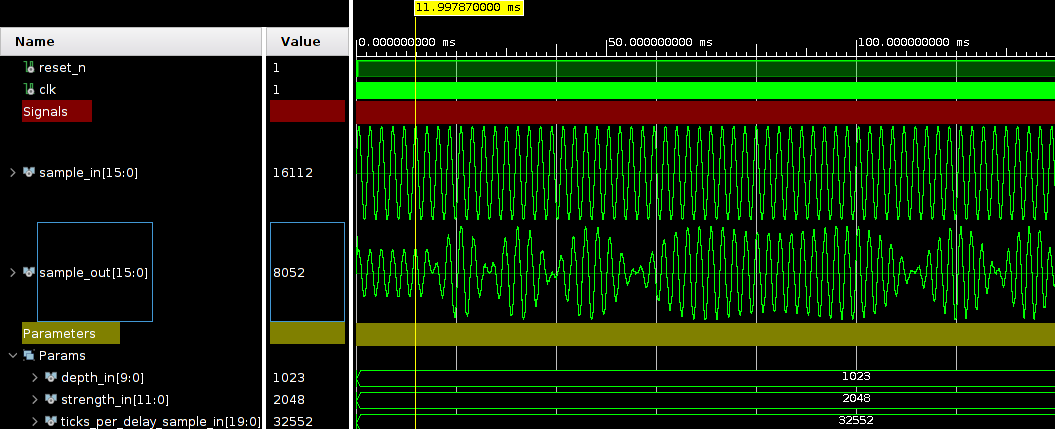
\includegraphics[width=\textwidth]{img/sim/flanger_sim.png}
    \captionsetup{format=plain,justification=centering}
    \caption{Fragment symulacji działania efektu \textit{flanger}}
    \label{sim-flanger}
\end{figure}
\vspace{0.5cm}
\section{Integracja potoku}

Po zakończeniu prac nad implementacją algorytmów przetwarzania przyszedł czas na ich zintegrowanie do postaci pojdeynczego modułu języka VHDL. Pierwszym krokiem do tak postawionego celu było ustalenie sposobu połączenia wszystkich efektów w~potok. Zdecydowano się na kolejność tremolo > delay > flanger > overdrive. Był to wybór raczej arbitralny wynikający z~braku doświadczenia autora w~dziedzinie projektowania filtrów cyfrowych. 

Kolejnym celem było ustalenie wartości parametrów poszczególnych efektów. W~celu ułatwienie późniejszych rekonfiguracji systemu stworzony został pakiet \verb|pipe_config| przechowujące stałe wykorzystywane do ich instancjonowania. W~przypadku efektu \textbf{overdrive} przyjęto szerokość wejścia \verb|gain|na poziomie $10$~bitów. Zastosowano także przesówanie wewnętrznego wyniku mnożenia o~$8$~bitów. Umożliwi to kontrolę wzmocnienia sygnały w~zakresie $[0,4)$ z~dokładnością ok. $0.39$\%. Efekt \textbf{tremolo} skonfigurowano do pracy z~generatorem fali trójkątnej o~$10$-bitowych próbkach. Szerokość wejścia \verb|depth| ustalono na $10$~bitów. Z~kolei szerokość wejścia \verb|period| określono na poziomie $17$~bitów. Pozwoli to na generowanie sygnału modulującego o~częstotliwości z~zakresu $[0.74,97000]$Hz. W~przypadku bloku \textbf{delay} zdecydowano się na wykorzystanie $12$-bitowego wejścia \verb|delay| oraz $16$-bitowego wejścia \verb|depth|. Parametry wykorzystannego do~jego regalizacji modułu BRAM opisano we wcześniejszej części dokumentu. Ostatni z~efektów - \textbf{flanger} - wymagał ustalenia wartości największej ilości parametrów. Szerokości wejść \verb|strength|, \verb|depth| i~\verb|period| ustawiono kolejno na $12$, $10$ i~$20$~bitów. Pozwoli to kontrolować siłę oraz amplitudę efektu z~dostateczną dokładnością a~jednocześnie zapewni częstotliwość LFO w~zakresie $[0.1,97000]$Hz. Warto zauważyć, że zakres ten jest zdecydowanie zbyt szeroki dla efektu \textit{flanger}. Aby zaprojektowany filtr mógł działać poprawnie częstotliwości te nie powinny przekraczać ok. $3$Hz (\cite{flanging_analysis}). Niedoskonałość ta wynika z~przyjętego sposobu okreslania okresu fali modulującej i~powinna zostać skorygowana na etapie podłączania wejścia \verb|period| do wyjścia interfejsu analogowego. Do relaizacji efektu \textit{flanger} wykorzystano dwa moduły BRAM. Pierwszy z~nich wykorzystywany jest przez generator fali sinusoidalnej. Przechowuje on $257$ równo oddalonych, $10$-bitowych próbek funkcji z~przedziału $[0,2\pi]$\footnote{Amplituda funkcji została rozszerzona do pełnego zakresu $10$-bitowej reprezentacji}. Przy próbkowaniu z~częstotliwością $44100$Hz pozwli to osiągnąć amplitudę opóźnień rzędu $23$ms. Blok zastosowany do buforowania danych wejściowych został z~kolei skonfigurowany do przechowywania $1024$ $16$-bitowych próbek, które mogą zostać zaadresowane przez wartości LFO.

Ostatnim krokiem na drodze do integracji potoku było odpowiednie przeskalowanie wejść parametryzujących poszczególne efektu w~celu uzyskania porządanych zakresów przy użyciu $12$-bitowej reprezentacji próbek wyjściowych interfejsu analogowego. Proces ten został szczegółowo opisany w~komentarzach kodu źródłowego potoku. W~tym miejscu warto zwrócić jedynie uwagę na fakt, że wejścia \verb|period| efektów \textit{tremolo} oraz \textit{flanger} zostały przeskalowane w~taki sposób aby zakres pozycji potencjometrów odpowiadał przedziałom $[0.74,94]$Hz dla pierwszego z~nich oraz $[0.1,3]$Hz dla drugiego. Tak skonstruowany potok został jeszcze raz poddany symulacji celem weryfikacji poprawności przepływu danych przez poszczególne segmenty. Fragment jej wyników ukazano na Rys. \ref{sim-pipe}.

\vspace{0.5cm}
\begin{figure}[ht]
    \centering
    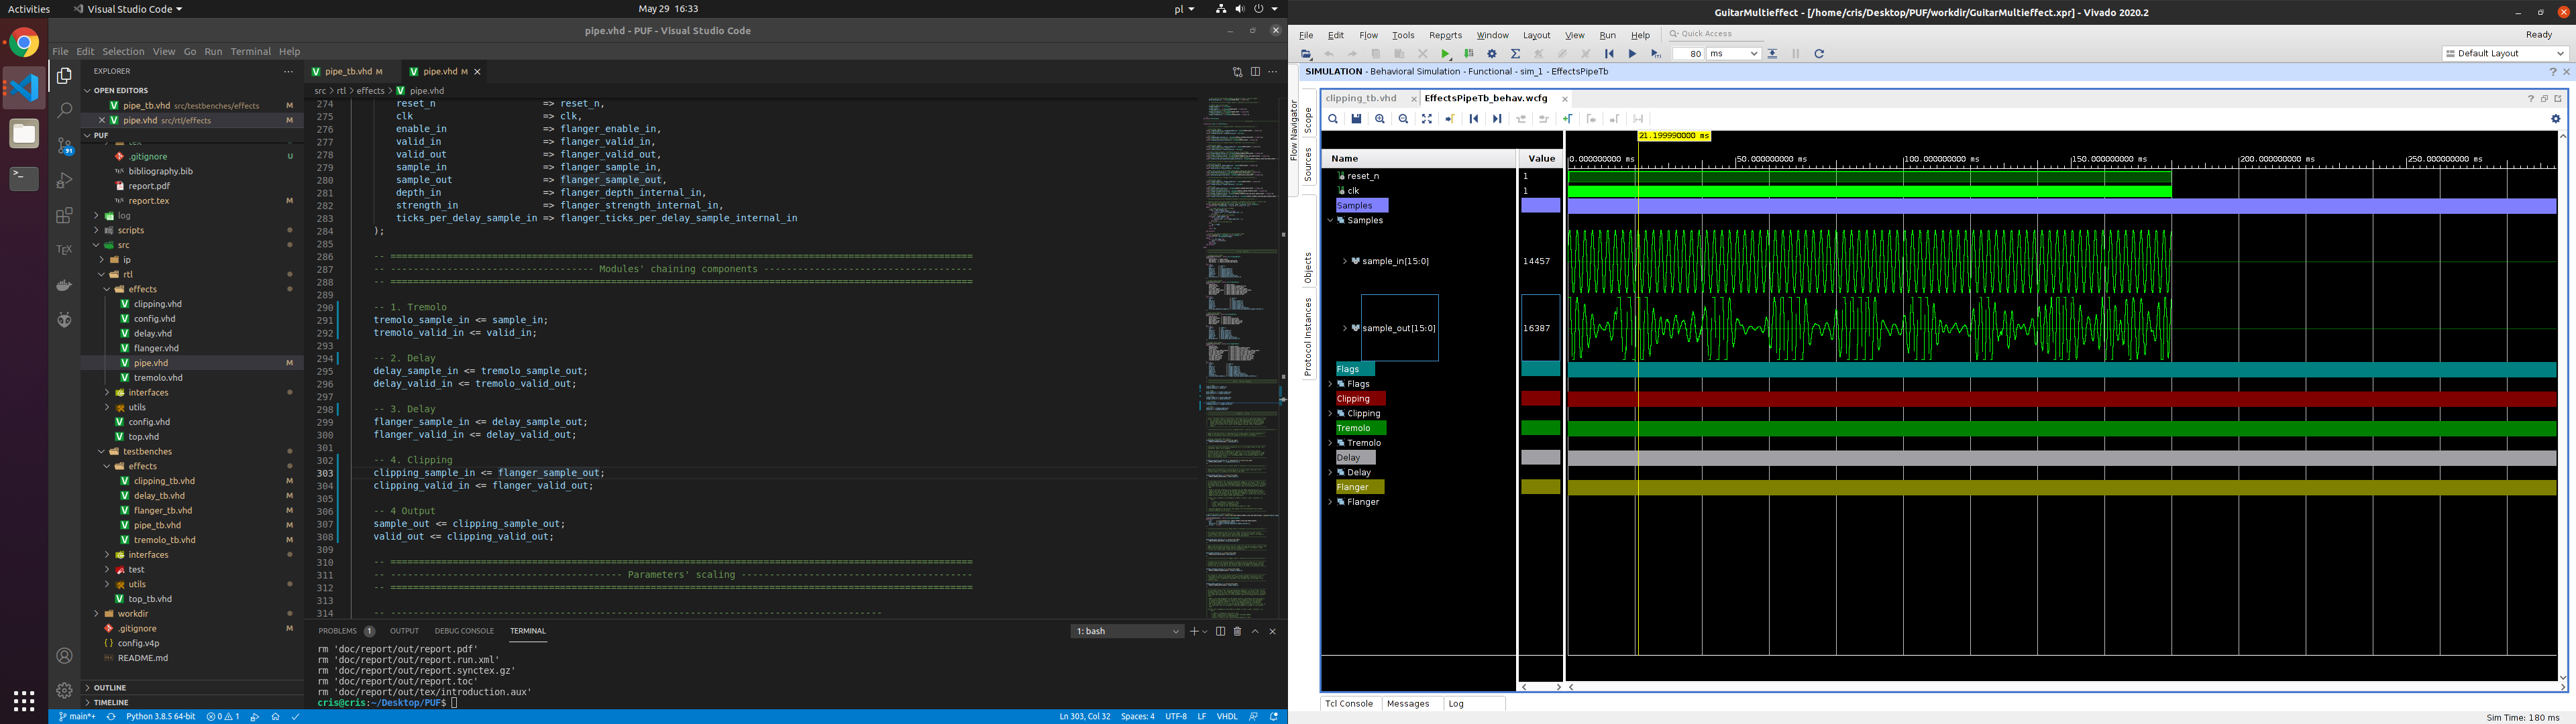
\includegraphics[width=\textwidth]{img/sim/pipe_sim.png}
    \captionsetup{format=plain,justification=centering}
    \caption{Fragment symulacji działania ostatecznego potoku efektów}
    \label{sim-pipe}
\end{figure}
\vspace{0.5cm}

\section{Integracja systemu}

Ostatecznym etapem projektu było połączenie stworzonych w~ten sposób modułów w~ramach pojedynczego bloku języka VHDL. Ze względu na regularne testowanie wdrażanych elementów oraz z~góry przemyślaną strukturę projektu proces ten przebiegł bezpoleśnie. Ostatecznie projekt udało się zsyntezować oraz przejść przez etap wirtualnej implementacji, czego efekt przedstawia Rys. \ref{synthesis}.

\vspace{1cm}
\begin{figure}[ht]
    \centering
    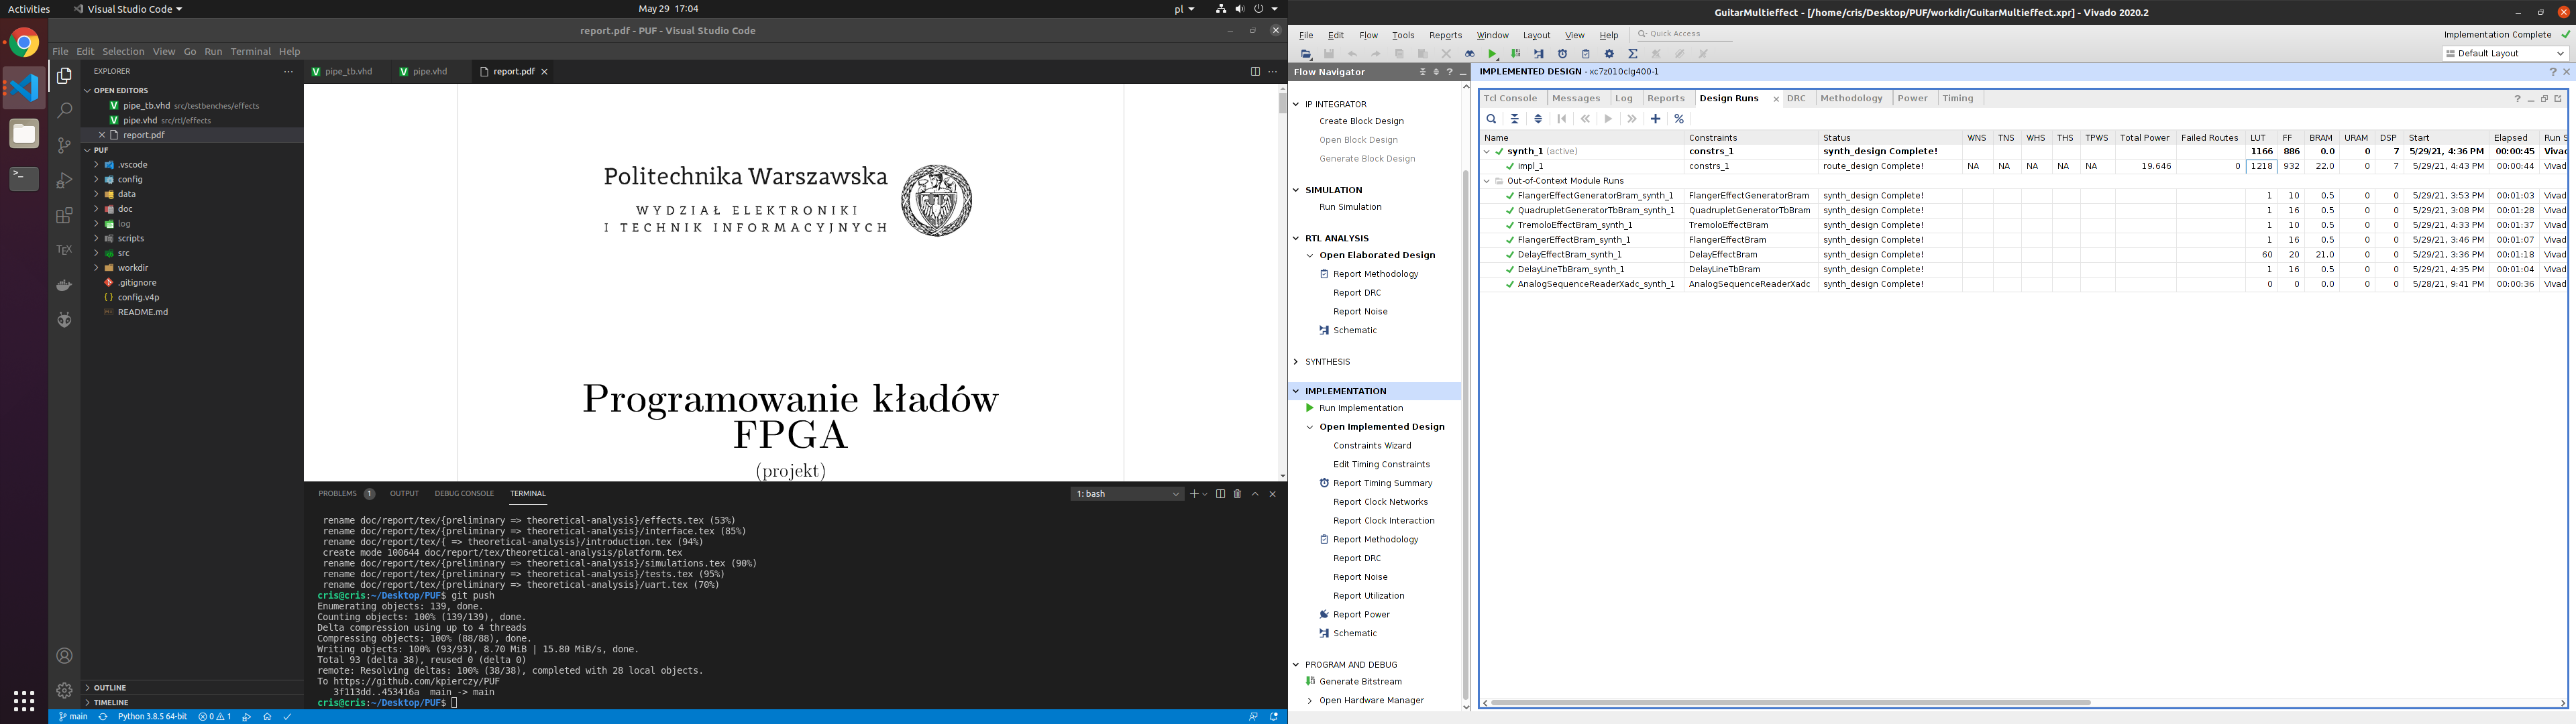
\includegraphics[width=\textwidth]{img/implementation.png}
    \captionsetup{format=plain,justification=centering}
    \caption{Efekt syntezy projektu}
    \label{synthesis}
\end{figure}
\vspace{1cm}

Niestety możliwość wykonania testów integracyjnych z~wykorzystaniem symulacji była dość ograniczona w~przypadku kompletnego projektu. Wynika to z~faktu, że parametry wszytskich efektów określane są przez wartości pobierane przez interfejs analogowy z~\textbf{pojedynczego} kanału XADC. Sposób symulacji XADC zaimplementowany w~\textit{Vivado} uniemożliwia zaimplementowanie wirtualnego multipleksera analogowego, który rozdzielałbym te sygnały. Wynika to z~faktu bezpośredniego podawania pobudzeń XADC na kanały modułu (brak możliwości zdefiniowania pobudzeń w~ramach testbencha). Przezwyciężenie tej trudności wymagałoby zmodyfikowania skryptu generującego plik z~przebiegami sygnałów analogowych w~taki sposób, aby uzględniał czasy próbkowania przetwornika ADC i~zapisywał wartości napięcia odpowiadające aktualnie odczytywanego parametru. Ze względu na i~tak już szeroki zakres projektu zrezygnowano z~realizji takiego podejścia.

W~zamian za to wykonano szereg symulacji obejmujących pełen tor przetwarzania (UART $\rightarrow$ Potok $\rightarrow$ UART), w~których parametry charakterystyczne poszczególnycyh efektów ustalane były poprzez sztucznie generowane przebiegi (zamiast poprzez moduł interfejsu analogowego). Pozwoliło to ostatecznie zweryfikować (przynajmniej od strony logicznej) poprawność działania zaprojektowanej konfiguracji FPGA. 

\vspace{0.75cm}
\begin{figure}[ht]
    \centering
    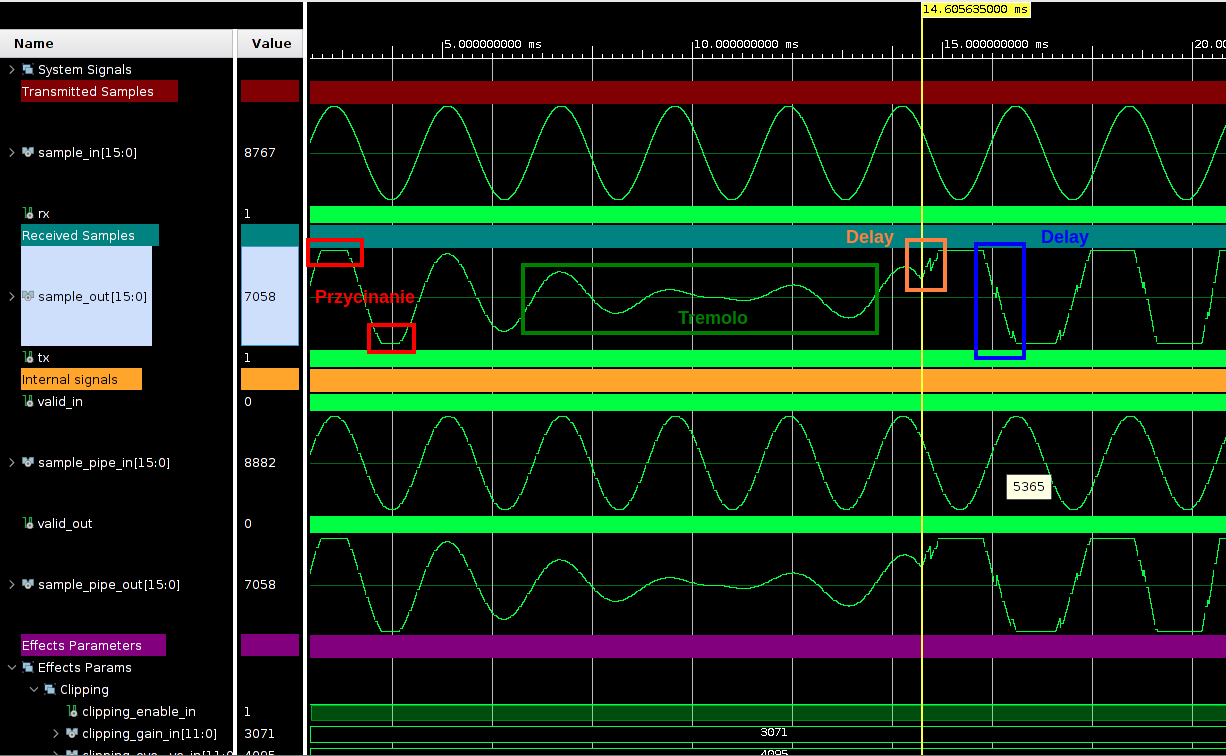
\includegraphics[width=\textwidth]{img/sim/top_all_effects_sim.png}
    \captionsetup{format=plain,justification=centering}
    \caption{Symulacja pełnego toru przetwarzania (wszystkie efekty aktywne)}
    \label{top-all-sim}
\end{figure}
\vspace{0.75cm}

Rys. \ref{top-all-sim} przedstawia symulację pełnego toru pomiarowego z~wszystkimi efektami w~stanie aktywnym. Tak jak w~przypadku poprzednich symulacji jako pobudzenie zastosowano falę sinusoidalną o~częstotliwości $440$Hz. Częstotliwość próbkowania wynosiła $44100$Hz. Sygnał \verb|sample_in| ukazuje pobudzenie wejścia urządzenia przesyłanego przez linię \verb|rx|. Z~kolei sygnał \verb|sample_out| to wyjście z~urządzenia odebrane przez jedną z~opisanych wcześniej funkcji bibliotecznych z~linii \verb|tx|. Dodatkowo zamieszczone zostały również przebiegi wewnętrznych (względem urządzenia) wartości wejściowej i~wyjściowej do potoku (t.j. wewnętrzne wyjście z~bloku odbierającego i~wejście do bloku transmitującego próbki). Na ukazanym przebiegu zaobserwować można efekty charakterystyczne dla każdgeo z~filtrów. W~pierwszej kolejności pojawia się przycinanie sygnału. Wzmocnienie modułu \textit{distortion} wynosiło $3$. W~następnej kolejności wkład do sygnału wyjściowego wnosi efekt termolo, który w~sposób cykliczny moduluje amplitudę wyjściową ze~współczynnikiem wzmocnienia w~zakresie $[0,1]$. Po $14.6$ms pojawia się skokowa zmiana sygnału wynikająca z~aktywacji modułu \textit{delay}, którego głębokość ustawiono na około $660$ próbek. Wpływ bloku \textit{flanger} nie jest tutaj widoczny, co wynika z~niewielkiego przedziału czasowego ukazanego na rysunku.

\section{Podsumowanie}

Zrealizowany projekt stanowił solidny wstęp do projektowania układów cyfrowych z~wykorzystaniem języka VHDL\footnote{W~niektórych kręgach można by nawet określić, że było to istny \textit{skok na głęboką wodę}.}. Pozwolił on nie tylko zapoznać się ze składnią języka w~stopniu umożliwiającym jego (stosunkowo) swobodne wykorzystywanie, ale także wdrożyć się w~sposób myślenia w~kategoriach konfiguracji zasobów sprzętowych tak różnego od tego, co znane jest z~tworzenia oprogramowania. Dodatkowym benefitem płynącym z~jego realizacji była możliwość poznania platformy projektowej w~postaci oprogramowania \textit{Vivado}, które umożliwi w~przyszłości znacznie szybsze zainicjalizowanie właściwej części prac nad nowymi projektami\footnote{Zapoznanie się z~rzeczonym oprogramowaniem utwierdziło także autora w~przekonaniu, że zintegrowane środowiska projektowe dostarczane przez dużych producentów nie są tym, co misie lubią najbardziej. W~przypadku przyszłych projektów duży nacisk zostanie położony na wykorzystanie skryptów języka \textit{Tcl}, które umożliwią jeszcze większą separację projektu od tego typu rozwiązań na rzecz środowiska stworzonego według własnych gustów i~przyzwyczajeń.}.

Ilość pracy włożonej w~projekt sprawiła, że stworzony w~jego ramach kod postanowiono doprowadzić do postaci, w~której będzie mógł on zostać wykorzystany z~autentycznym sprzętem gitarowym. Wymagać to będzie stworzenia odpowiedniej platformy sprzętowej. Zadanie to obejmuje określenie wykorzystanych komponentów (ze szczególnym uwzględnieniem elementów analogowych) oraz (potencjalnie) zaprojektowanie własnego obwodu drukowanego. Na dzień dzisiejszy prace te zostają odłożone w~czasie do momentu ukończenia projektów realizowany w~ramach jakże służnie mijającego semestru.


\part{Dodatek - opisy wyprowadzeń modułów}

% ================================================================================================================================== %
% -------------------------------------------------------- Serial interface -------------------------------------------------------- %
% ================================================================================================================================== %

\begin{table}[h]
\small
\centering
\begin{tabular}{|c|l|c|c|c|m{4.5cm}|}
\hline
\rowcolor[HTML]{C0C0C0}
\textbf{Np.} & \textbf{Nazwa} & \textbf{Typ} & \textbf{Stan aktywny} & \textbf{Rozmiar} & \textbf{Opis}                                                                                                                                      \\ \hline
\rowcolor[HTML]{F8A102}\multicolumn{6}{|l|}{Układ odbierający UART} \\ \hline
1            & clk            & in           & zbocze narastające    & 1                & Sygnał taktujący                                                                                                                                   \\ \hline
2            & reset          & in           & niski                 & 1                & Sygnał resetujący                                                                                                                                  \\ \hline
3            & rate           & in           & N/D                   & P                & Okres pojedynczego bitu odbieranego wyrażany jako ilość taktów zegara systemowego (clk) minus~1; gdy ustawiony na 0, układ przestaje odbierać dane \\ \hline
4            & rx             & in           & P                     & 1                & Szeregowe wejście danych                                                                                                                           \\ \hline
5            & busy           & out          & wysoki                & 1                & Sygnał wskazujący, że układ znajduje się w~stanie odbierania                                                                                       \\ \hline
6            & error          & out          & wysoki                & 3                & Flagi błędów odbioru (bitów start/stopu) oraz błędu parzystości                                                                                    \\ \hline
7            & data           & out          & N/D                   & P ($5-8$)        & Równoległe wyjście odebranych danych                                                                                                               \\ \hline
\multicolumn{6}{|l|}{\cellcolor[HTML]{F8A102}Układ nadający UART} \\ \hline
1            & clk            & in           & zbocze narastające    & 1                & Sygnał taktujący                                                                                                                                   \\ \hline
2            & reset          & in           & niski                 & 1                & Sygnał resetujący                                                                                                                                  \\ \hline
3            & rate           & in           & N/D                   & P                & Okres pojedynczego bitu odbieranego wyrażany jako ilość taktów zegara systemowego (clk) minus~1                                                    \\ \hline
5            & transfer       & in           & wysoki                & 1                & Sygnał aktywujący transfer danych z~linii \textit{data}                                                                                            \\ \hline
7            & data           & in           & N/D                   & P (5-8)          & Równoległe wejście danych                                                                                                                          \\ \hline
6            & busy           & out          & wysoki                & 1                & Sygnał wskazujący, że układ znajduje się w~stanie nadawanie                                                                                        \\ \hline
8            & tx             & out          & P                     & 1                & Szeregowe wyjście danych                                                                                                                           \\ \hline 
\multicolumn{6}{|l|}{\cellcolor[HTML]{F8A102}Układ odbierający próbki} \\ \hline
1            & clk            & in           & zbocze narastające    & 1                & Sygnał taktujący                                                                                                                                   \\ \hline
2            & reset          & in           & niski                 & 1                & Sygnał resetujący                                                                                                                                  \\ \hline
4            & rx             & in           & P                     & 1                & Szeregowe wejście danych                                                                                                                           \\ \hline
5            & busy           & out          & wysoki                & 1                & Sygnał wskazujący, że układ znajduje się w~stanie odbierania                                                                                       \\ \hline
6            & err            & out          & wysoki                & 3                & Flagi błędów odbioru (bitów start/stopu) oraz błędu parzystości                                                                                    \\ \hline
7            & sample         & out          & N/D                   & P ($8n$)         & Równoległe wyjście odebranych danych                                                                                                               \\ \hline
\end{tabular}
\caption{Wyprowadzenia modułów}
\end{table}

% Continued
\setcounter{table}{0}
\begin{table}[t]
\small
\centering
\begin{tabular}{|c|l|c|c|c|m{4.5cm}|}
\hline
\rowcolor[HTML]{C0C0C0}
\textbf{Np.} & \textbf{Nazwa} & \textbf{Typ} & \textbf{Stan aktywny} & \textbf{Rozmiar} & \textbf{Opis}                                                      \\ \hline
\multicolumn{6}{|l|}{\cellcolor[HTML]{F8A102}Układ nadający próbki} \\ \hline
1            & clk            & in           & zbocze narastające    & 1                & Sygnał taktujący                                                   \\ \hline
2            & reset          & in           & niski                 & 1                & Sygnał resetujący                                                  \\ \hline
3            & transfer       & in           & wysoki                & 1                & Sygnał aktywujący transfer danych z~linii \textit{data}            \\ \hline
4            & sample         & in           & N/D                   & P ($8n$)         & Równoległe wejście danych                                          \\ \hline
5            & busy           & out          & wysoki                & 1                & Sygnał wskazujący, że układ znajduje się w~stanie nadawanie        \\ \hline
6            & tx             & out          & P                     & 1                & Szeregowe wyjście danych                                           \\ \hline
\rowcolor[HTML]{32CB00}\multicolumn{6}{|l|}{Moduł analogowy} \\ \hline
1            & clk            & in           & zbocze narastające    & 1                 & Sygnał taktujący                                                  \\ \hline
2            & reset          & in           & niski                 & 1                 & Sygnał resetujący                                                 \\ \hline
3            & analog+        & in           & N/D                   & 1                 & Dodatni terminal wejścia analogowego                              \\ \hline
4            & analog-        & in           & N/D                   & 1                 & Ujemny terminal wejścia analogowego                               \\ \hline
5            & mux\_select    & out          & N/D                   & 4                 & Sygnał \textit{select} dla zewnętrznego multipleksera analogowego \\ \hline
\rowcolor[HTML]{34CDF9}\multicolumn{6}{|l|}{Efekt \textit{overdiver}} \\ \hline
1            & clk            & in           & zbocze narastające    & 1                 & Sygnał taktujący                                                  \\ \hline
2            & reset\_n       & in           & niski                 & 1                 & Sygnał resetujący                                                 \\ \hline
3            & enable\_in     & in           & wysoki                & 1                 & Aktywacja efektu                                                  \\ \hline
4            & valid\_in      & in           & wysoki                & 1                 & Sygnał aktywujący przetworzenie danych wejściowych                \\ \hline
5            & sample\_in     & in           & N/D                   & P ($8n$)          & Wejście danych                                                    \\ \hline
6            & valid\_out     & out          & wysoki                & 1                 & Sygnał oznaczający wystawienie przetworzonych danych na wyjście   \\ \hline
7            & sample\_out    & out          & N/D                   & P ($8n$)          & Wyjście danych                                                    \\ \hline
8            & gain           & in           & N/D                   & P                 & Wzmocnienie sygnału wejściowego                                   \\ \hline
9            & saturation     & in           & N/D                   & P ($8n-1$)        & Poziom nasycenia sygnału wyjściowego                              \\ \hline
\end{tabular}
\caption{Wyprowadzenia modułów (kontunuacja)}
\end{table}

% Continued
\setcounter{table}{0}
\begin{table}[t]
\small
\centering
\begin{tabular}{|c|l|c|c|c|m{4.5cm}|}
\hline
\rowcolor[HTML]{C0C0C0}
\textbf{Np.} & \textbf{Nazwa} & \textbf{Typ} & \textbf{Stan aktywny} & \textbf{Rozmiar} & \textbf{Opis} \\ \hline
\rowcolor[HTML]{34CDF9}\multicolumn{6}{|l|}{Efekt tremolo} \\ \hline
1            & clk       & in           & zbocze narastające    & 1                 & Sygnał taktujący                                                                                                           \\ \hline
2            & reset     & in           & niski                 & 1                 & Sygnał resetujący                                                                                                          \\ \hline
3            & enable    & in           & wysoki                & 1                 & Aktywacja efektu                                                                                                           \\ \hline
4            & valid in  & in           & wysoki                & 1                 & Sygnał aktywujący przetworzenie danych wejściowych                                                                         \\ \hline
5            & in data   & in           & N/D                   & P ($8n$)          & Wejście danych                                                                                                             \\ \hline
6            & valid out & out          & wysoki                & 1                 & Sygnał oznaczający wystawienie przetworzonych danych na wyjście                                                            \\ \hline
7            & out data  & out          & N/D                   & P ($8n$)          & Wyjście danych                                                                                                             \\ \hline
8            & depth     & in           & N/D                   & P                 & Głębokość efektu rozumiana jako parametr $d$ równania $y[t] = 1 - d \times x[t]$ wyznaczającego poziom modulacji           \\ \hline
9            & period    & in           & N/D                   & P ($8n-1$)        & Ilość taktów zegara systemowego przypadających na jedną próbkę sygnału modulującego                                        \\ \hline
\rowcolor[HTML]{34CDF9}\multicolumn{6}{|l|}{Efekt \textit{delay}} \\ \hline
1            & clk       & in           & zbocze narastające    & 1                 & Sygnał taktujący                                                                                                           \\ \hline
2            & reset     & in           & niski                 & 1                 & Sygnał resetujący                                                                                                          \\ \hline
3            & enable    & in           & wysoki                & 1                 & Aktywacja efektu                                                                                                           \\ \hline
4            & valid in  & in           & wysoki                & 1                 & Sygnał aktywujący przetworzenie danych wejściowych                                                                         \\ \hline
5            & in data   & in           & N/D                   & P ($8n$)          & Wejście danych                                                                                                             \\ \hline
6            & valid out & out          & wysoki                & 1                 & Sygnał oznaczający wystawienie przetworzonych danych na wyjście                                                            \\ \hline
7            & out data  & out          & N/D                   & P ($8n$)          & Wyjście danych                                                                                                             \\ \hline
8            & delay     & in           & N/D                   & P                 & Głębokość echa rozumiana jako odległość (wyrażona w~czasie dyskretnym między próbką wejściową a~próbką z~nią sumowaną)     \\ \hline
8            & depth     & in           & N/D                   & P                 & Wzmocnienie opóźnionej części sygnału wyjściowego                                                                          \\ \hline
\end{tabular}
\caption{Wyprowadzenia modułów (kontunuacja)}
\end{table}

% Continued
\setcounter{table}{0}
\begin{table}[t]
\small
\centering
\begin{tabular}{|c|l|c|c|c|m{4.5cm}|}
\hline
\rowcolor[HTML]{C0C0C0}
\textbf{Np.} & \textbf{Nazwa} & \textbf{Typ} & \textbf{Stan aktywny} & \textbf{Rozmiar} & \textbf{Opis} \\ \hline
\rowcolor[HTML]{34CDF9}\multicolumn{6}{|l|}{Efekt \textit{flanger}} \\ \hline
1            & clk       & in           & zbocze narastające    & 1                 & Sygnał taktujący                                                                                                           \\ \hline
2            & reset     & in           & niski                 & 1                 & Sygnał resetujący                                                                                                          \\ \hline
3            & enable    & in           & wysoki                & 1                 & Aktywacja efektu                                                                                                           \\ \hline
4            & valid in  & in           & wysoki                & 1                 & Sygnał aktywujący przetworzenie danych wejściowych                                                                         \\ \hline
5            & in data   & in           & N/D                   & P ($8n$)          & Wejście danych                                                                                                             \\ \hline
6            & valid out & out          & wysoki                & 1                 & Sygnał oznaczający wystawienie przetworzonych danych na wyjście                                                            \\ \hline
7            & out data  & out          & N/D                   & P ($8n$)          & Wyjście danych                                                                                                             \\ \hline
8            & depth     & in           & N/D                   & P                 & Głębokość efektu rozumiana jako amlituda opóźnień opóźnionej części sygnału wyjściowego                                    \\ \hline
8            & strength  & in           & N/D                   & P                 & Udział sygnału opóźnionego w~sygnale wyjściowym                                                                            \\ \hline
8            & period    & in           & N/D                   & P                 & Okres oscylacji opóźnienia wyrażony w~ilości taktów zegara systemowego przypadajacych na jedną próbkę sygnału oscylującego \\ \hline
\end{tabular}
\caption{Wyprowadzenia modułów (kontunuacja)}
\end{table}



% Bibliography
\clearpage
\printbibliography

\end{document}


